%%
%% Copyright 2007, 2008, 2009 Elsevier Ltd
%%
%% This file is part of the 'Elsarticle Bundle'.
%% ---------------------------------------------
%%
%% It may be distributed under the conditions of the LaTeX Project Public
%% License, either version 1.2 of this license or (at your option) any
%% later version.  The latest version of this license is in
%%    http://www.latex-project.org/lppl.txt
%% and version 1.2 or later is part of all distributions of LaTeX
%% version 1999/12/01 or later.
%%
%% The list of all files belonging to the 'Elsarticle Bundle' is
%% given in the file `manifest.txt'.
%%

%% Template article for Elsevier's document class `elsarticle'
%% with numbered style bibliographic references
%% SP 2008/03/01

\documentclass[preprint,1p]{elsarticle}
\biboptions{numbers,sort&compress}

%% Use the option review to obtain double line spacing
%% \documentclass[authoryear,preprint,review,12pt]{elsarticle}

%% Use the options 1p,twocolumn; 3p; 3p,twocolumn; 5p; or 5p,twocolumn
%% for a journal layout:
%% \documentclass[final,1p,times]{elsarticle}
%% \documentclass[final,1p,times,twocolumn]{elsarticle}
%% \documentclass[final,3p,times]{elsarticle}
%% \documentclass[final,3p,times,twocolumn]{elsarticle}
%% \documentclass[final,5p,times]{elsarticle}
%% \documentclass[final,5p,times,twocolumn]{elsarticle}

%% For including figures, graphicx.sty has been loaded in
%% elsarticle.cls. If you prefer to use the old commands
%% please give \usepackage{epsfig}

%% The amssymb package provides various useful mathematical symbols

\usepackage{amssymb}
\usepackage{lineno}
\usepackage{hyperref}
\usepackage{siunitx}
\usepackage{multirow}
\usepackage{wasysym}
\usepackage{tabularx}
%\usepackage{mathtools}
\usepackage{xcolor}
\usepackage{booktabs,multirow}%
\newcommand{\makecell}[2][@{}c@{}]{\begin{tabular}{#1}#2\end{tabular}}

%\usepackage[margin=1in]{geometry}% Just for this example
%\usepackage[percent]{overpic}
%\usepackage[usenames,dvipsnames,svgnames,table]{xcolor}
%\usepackage{cleveref}

%% The amsthm package provides extended theorem environments
%% \usepackage{amsthm}

%% The lineno packages adds line numbers. Start line numbering with
%% \begin{linenumbers}, end it with \end{linenumbers}. Or switch it on
%% for the whole article with \linenumbers.
%% \usepackage{lineno}

\journal{Nucl. Instrum. Meth. A}

\begin{document}

\linenumbers

\begin{frontmatter}

%% Title, authors and addresses

%% use the tnoteref command within \title for footnotes;
%% use the tnotetext command for theassociated footnote;
%% use the fnref command within \author or \address for footnotes;
%% use the fntext command for theassociated footnote;
%% use the corref command within \author for corresponding author footnotes;
%% use the cortext command for theassociated footnote;
%% use the ead command for the email address,
%% and the form \ead[url] for the home page:
%% \title{Title\tnoteref{label1}}
%% \tnotetext[label1]{}
%% \author{Name\corref{cor1}\fnref{label2}}
%% \ead{email address}
%% \ead[url]{home page}
%% \fntext[label2]{}
%% \cortext[cor1]{}
%% \address{Address\fnref{label3}}
%% \fntext[label3]{}

\title{A simulation model of front-end electronics for high-precision timing measurements with low-gain avalanche detectors.}

%% use optional labels to link authors explicitly to addresses:
%% \author[label1,label2]{}
%% \address[label1]{}
%% \address[label2]{}

\author[1,2]{C.~Pe\~na\corref{cor}}\ead{cmorgoth@fnal.gov}
\author[1]{G.~Deptuch}
\author[2]{S.~Xie}
\author[1]{A.~Apresyan}
\author[2]{L.~Narv\'aez}
\author[1]{T.~Liu}
\author[3]{N.~Cartiglia}


\address[1]{Fermi National Accelerator Laboratory, Batavia, IL, USA}
\address[2]{California Institute of Technology, Pasadena, CA, USA}
\address[3]{INFN, Torino, Italy}
\cortext[cor]{Corresponding author}

\begin{abstract}
%% Text of abstract
In this paper we report simulation results of a study aiming to optimize 
parameters of a detector that uses low-gain avalanche detectors (LGAD) for
high-precision timing measurements. The detector is assumed to be composed of a
50~$\mu$m LGAD sensor coupled to front-end readout electronics which is used to
measure the time of arrival of minimum ionizing particles. The simulation
includes modeling of signal fluctuations in the LGAD sensor, variations of the analog
bandwidth and signal-to-noise ratio (SNR) of the front-end electronics, time
bin quantization, and radiation damage of the LGAD sensors. Two approaches to
measure the timestamp are considered: leading edge and constant fraction.
Simulated LGAD pulses before irradiation, and after irradiation with 
neutron fluences of $5\times 10^{14}$~n/cm$^2$ and $1\times 10^{15}$~n/cm$^2$,
are studied. The time resolution for a 50~$\mu$m LGADs was found to be ~35~\si{ps}
for front-end electronics bandwidths larger than 350~\si{MHz} and SNRs larger
than 30. The time resolution at SNR of 30 for fluences of $5\times
10^{14}$~n/cm$^2$ and $1\times 10^{15}$~n/cm$^2$ were found to be ~31~\si{ps}
and ~37~\si{ps}, respectively. 
\end{abstract}

\begin{keyword}
%% keywords here, in the form: keyword \sep keyword

%% PACS codes here, in the form: \PACS code \sep code
Silicon \sep Timing \sep LGAD
%% MSC codes here, in the form: \MSC code \sep code
%% or \MSC[2008] code \sep code (2000 is the default)

\end{keyword}

\end{frontmatter}

\tableofcontents

%% \linenumbers

%% main text
\section{Introduction}

Low-gain avalanche diodes (LGAD) are envisioned to be used in the CMS and ATLAS experiment 
upgrades for HL-LHC in order to overcome event reconstruction challenges posed by the high rate of concurrent
collisions per beam crossing (pileup). The instrumented regions of pseudorapidity ($\eta$)
are: $1.6< |\eta| <2.9$, and $2.4< |\eta|<4.2$ for CMS and ATLAS, respectively.
Beam test measurements have demonstrated that the required time resolution,
radiation tolerance, and uniformity of LGAD sensors can be achieved~\cite{Apresyan:2018oln,Allaire_2018}.

In this paper we report simulation results of a study aiming to optimize 
parameters of a detector that uses 50~$\mu$m low-gain avalanche detectors (LGAD) for
high-precision timing measurements. The simulation model include effects due to variations 
in LGAD signal pulse shape and amplitude, different analog bandwidth and signal-to-noise ratio (SNR) of the front-end readout 
electronics (FEE), time bin quantization, and radiation damage on LGAD sensors.
We scan the important parameters for time resolution: analog bandwidths (BWs),
signal-to-noise ratios (SNR), and the total neutron equivalent fluence that the 
LGAD sensor has been subjected to. Our results indicate that for FEE analog BWs larger than 350~\si{MHz},
corresponding to shaping times less than 1~\si{ns} and SNR larger than 30, time resolutions of 30--37~\si{ps} and 34--47~\si{ps}
are obtained when using constant fraction (CF) and leading edge (LE) discriminators in their ideal mathematical implementations, respectively.
These results are compatible with previous measurements on LGAD timing resolutions carried out under
laboratory and beam test conditions~\cite{Apresyan:2018oln, Cartiglia201783, PELLEGRINI201412}.
We study the time resolution of four different FEE shaping times: $0.5$, $1.0$,
$2.0$, and $4.0$~\si{ps}; three SNR: 20, 30, 100; and three sensor irradiation
levels: pre-radiation, $5\times 10^{14}$~n/cm$^2$, and $1\times 10^{15}$~n/cm$^2$.
For every point in this scan we evaluate the time resolution for LE and CF.
Our results are a guideline on what time resolution can
be achieved for a particular combination of analog bandwidth, SNR, and sensor.

The paper is organized as follows: the simulation is described in
Sec.~\ref{sec:simulation}; algorithms used in the timing
reconstruction and analysis are described in Sec.~\ref{sec:timing_and_analysis}; simulation results
are presented in Sec.~\ref{sec:results}, followed by the conclusion in
Sec.~\ref{sec:conclusion}.

\section{Simulation Framework}
\label{sec:simulation}

Unprocessed signal pulses from the LGAD sensors are obtained from Weightfield2
(WF2), a 2-dimensional silicon simulator~\cite{Sadrozinski:2017qpv}. WF2 was
used to simulate sets of 1000 signal pulses modeling the response off
minimum-ionizing particles (MIP) traversing the LGAD sensor, and the MIP
impinges on the LGAD perpendicularly to its surface. Three sets of such signal
pulses were generated for a 50~$\mu$m LGAD sensor at different levels of sensor
irradiation: pre-irradiation, and after neutron fluences of $5\times
10^{14}$~n/cm$^2$ and $1\times 10^{15}$~n/cm$^2$. Fig.~\ref{fig:lgad_current} shows the
unprocessed LGAD output current from WF2 for 1000 signal pulses (left)
and example pulses for all the irradiation levels studied (right).
Gaussian white noise is added later
to these unprocessed signals, and the combined waveform is fed into the
simulation of the FEE. The schematic diagram of the data flow is illustrated
in Fig.~\ref{fig:simulation_diagram} and described in further detail in
Sec.~\ref{sub_sec:fee_simulation_and_noise}. The output of the FEE simulation is
the convolution of the impulse response function and the input signal at the
FEE~\cite{Sansen}. We consider four time constants for the impulse response of the FEE:
0.5, 1.0, 2.0, and 4.0~\si{ns}. At the output of the FEE block, we obtain
simulated processed LGAD pulses, which include the effects of sensor
fluctuations, the shaping of the FEE, and noise. The resulting processed pulses
are scaled such that the most probable value (MPV) for each of the simulated conditions is 50~\si{mV}.
This choice of normalization does not affect the time resolution results since the SNR is
maintained. By enforcing the same normalization for every simulation condition
 we ensure that the LE thresholds occur at the same proportion to the pulse maximum. 


 \begin{figure}[htbp]
   \centering
   \includegraphics[width=0.48\textwidth]{figs/lgad_current_pre_rad_all_pulses_v2.pdf} \hfill
   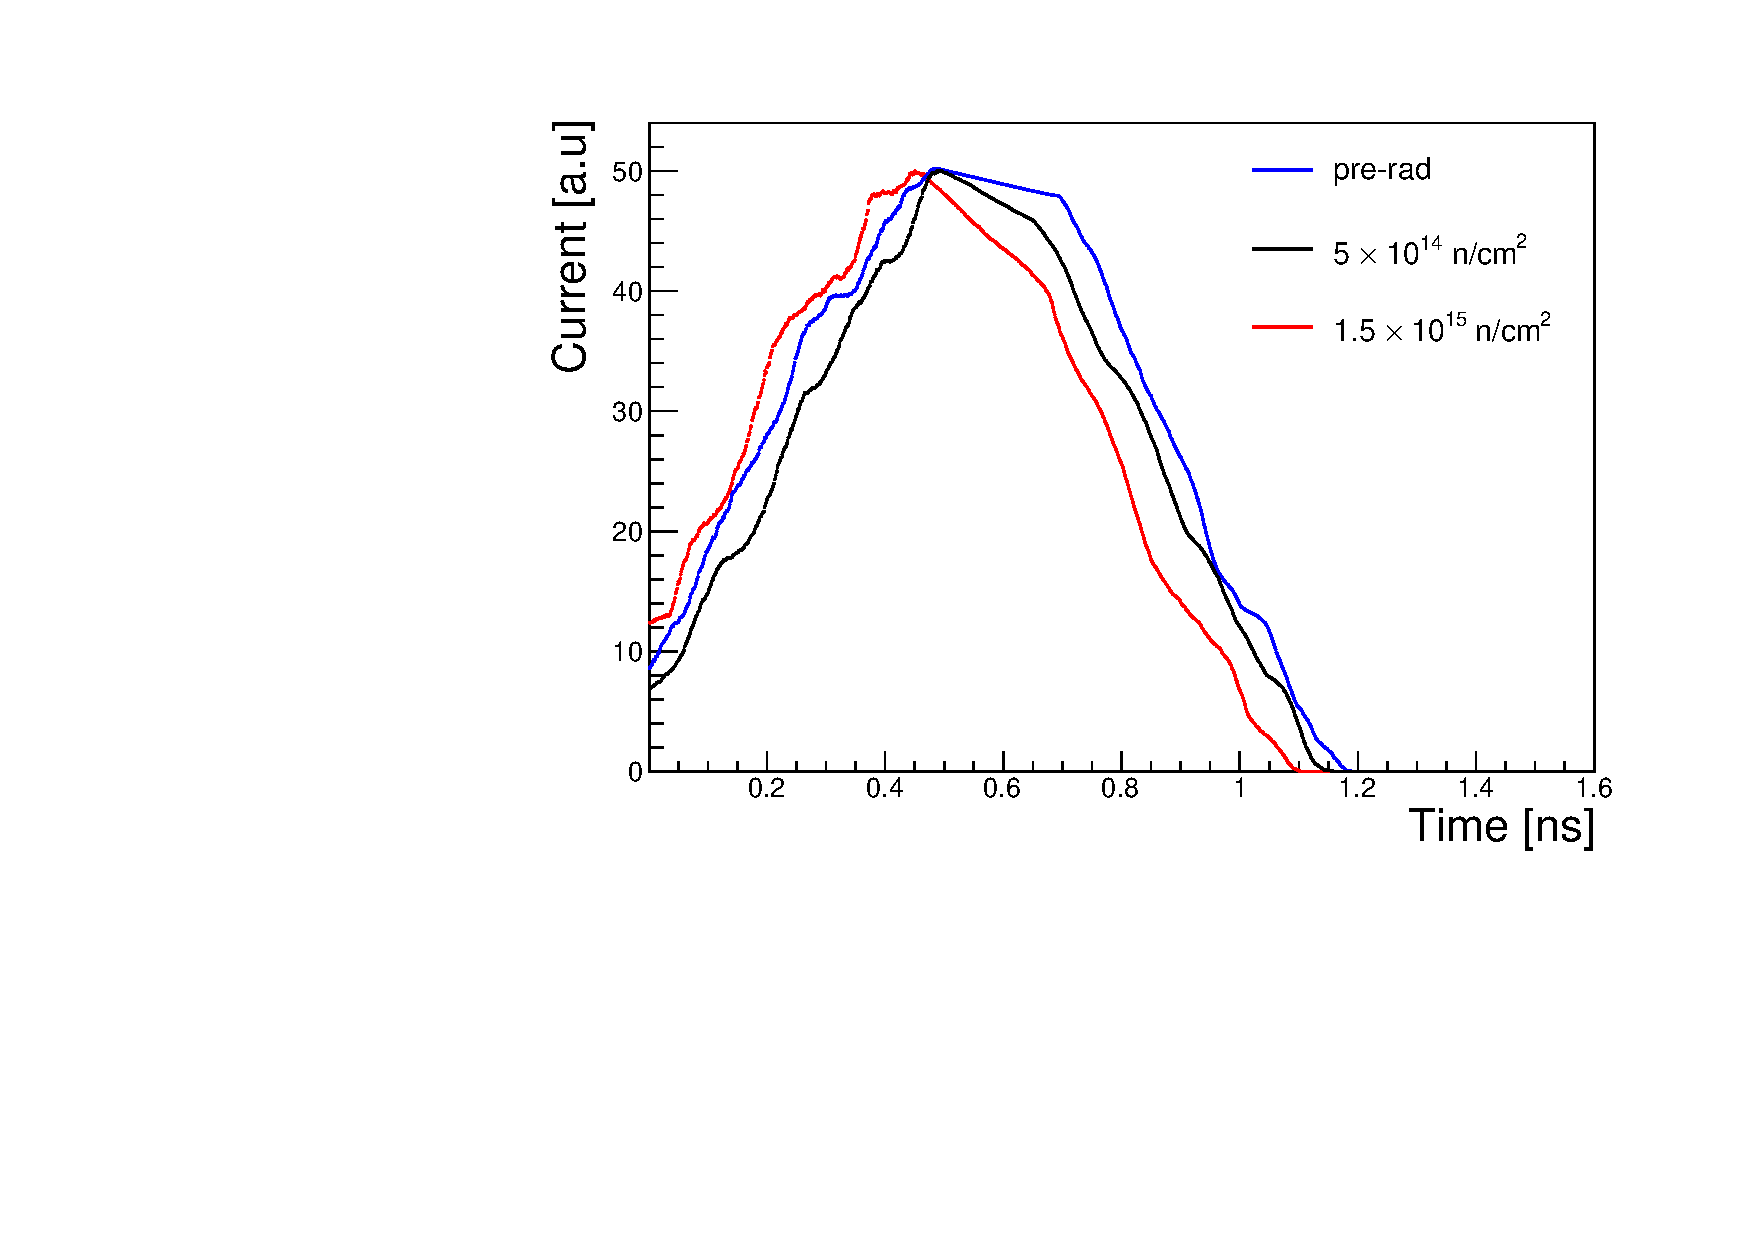
\includegraphics[width=0.48\textwidth]{figs/LGAD_current_all_irradiations_v2.pdf}
   \caption{(Left) One thousand LGAD output current pulses from WF2 for a pre-radiation sensor.
   (Right) Example LGAD output current pulses for different irradiation levels.}
   \label{fig:lgad_current}
 \end{figure}


A waveform analysis is performed with the pulses obtained at the output of the
FEE block. We assign timestamps to each pulse by using algorithms that emulate
ideal LE and CF discriminators. For each threshold we obtain an LE and CF
timestamp as well as the corresponding time-over-theshold (ToT) of the pulse.
The SNR is defined as the ratio of the MPV of the amplitude distribution to the
r.m.s of the amplitude distribution of sampled noise-only waveforms.
Fig.~\ref{fig:amp_and_noise} shows the amplitude distribution and the respective Landau fit
from where the MPV is obatained (left) and the amplitude distribution for a fixed sample (right)
for a pre-radiation sensor with a SNR of 30.
We study three SNR scenarios: 20, 30, and 100. A schematic diagram of the
simulation is shown in Fig.~\ref{fig:simulation_diagram}.



%This simulation
% implements a more
% realistic version of a CF discriminator
%based on signal delays.
\begin{figure}[htbp]
  \centering
  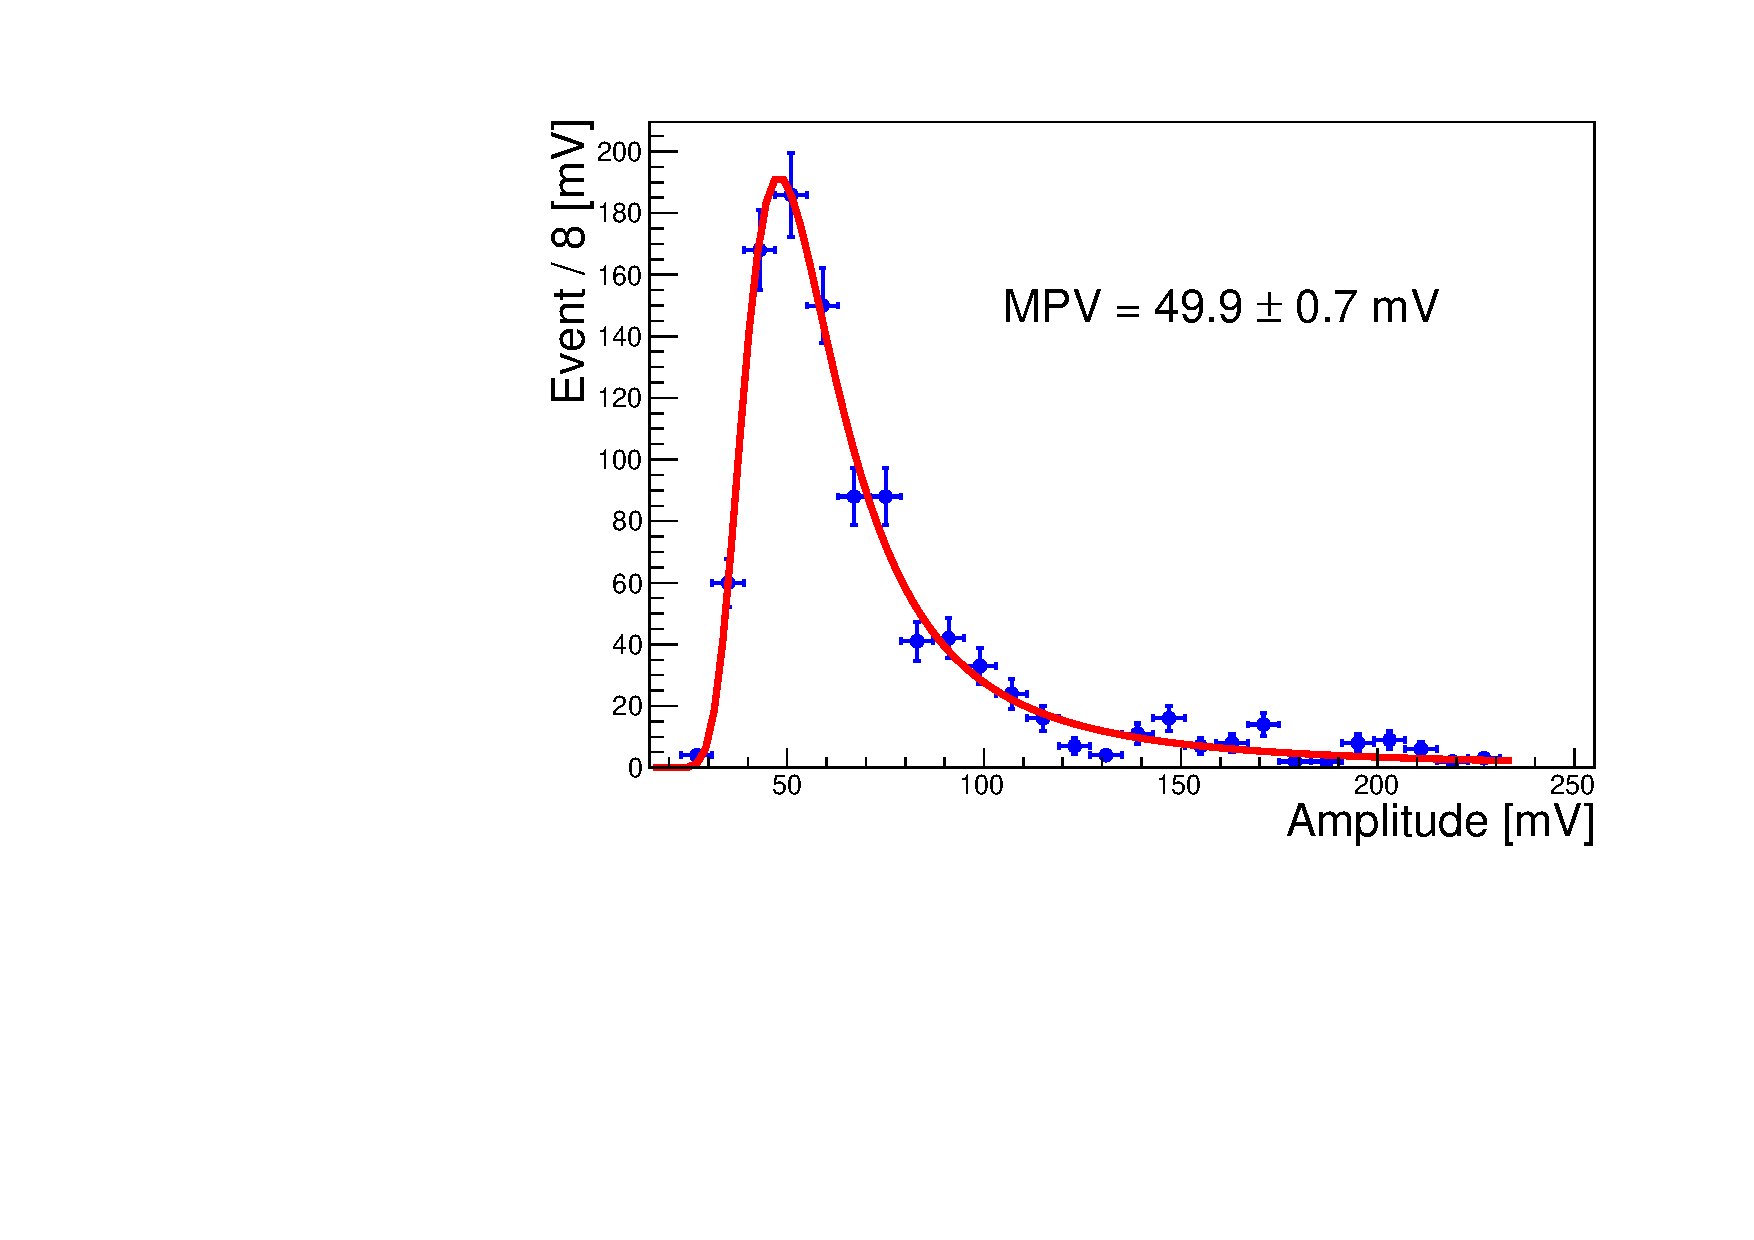
\includegraphics[width=0.48\textwidth]{figs/amplitude_1ns_landau_fit.pdf} \hfill
  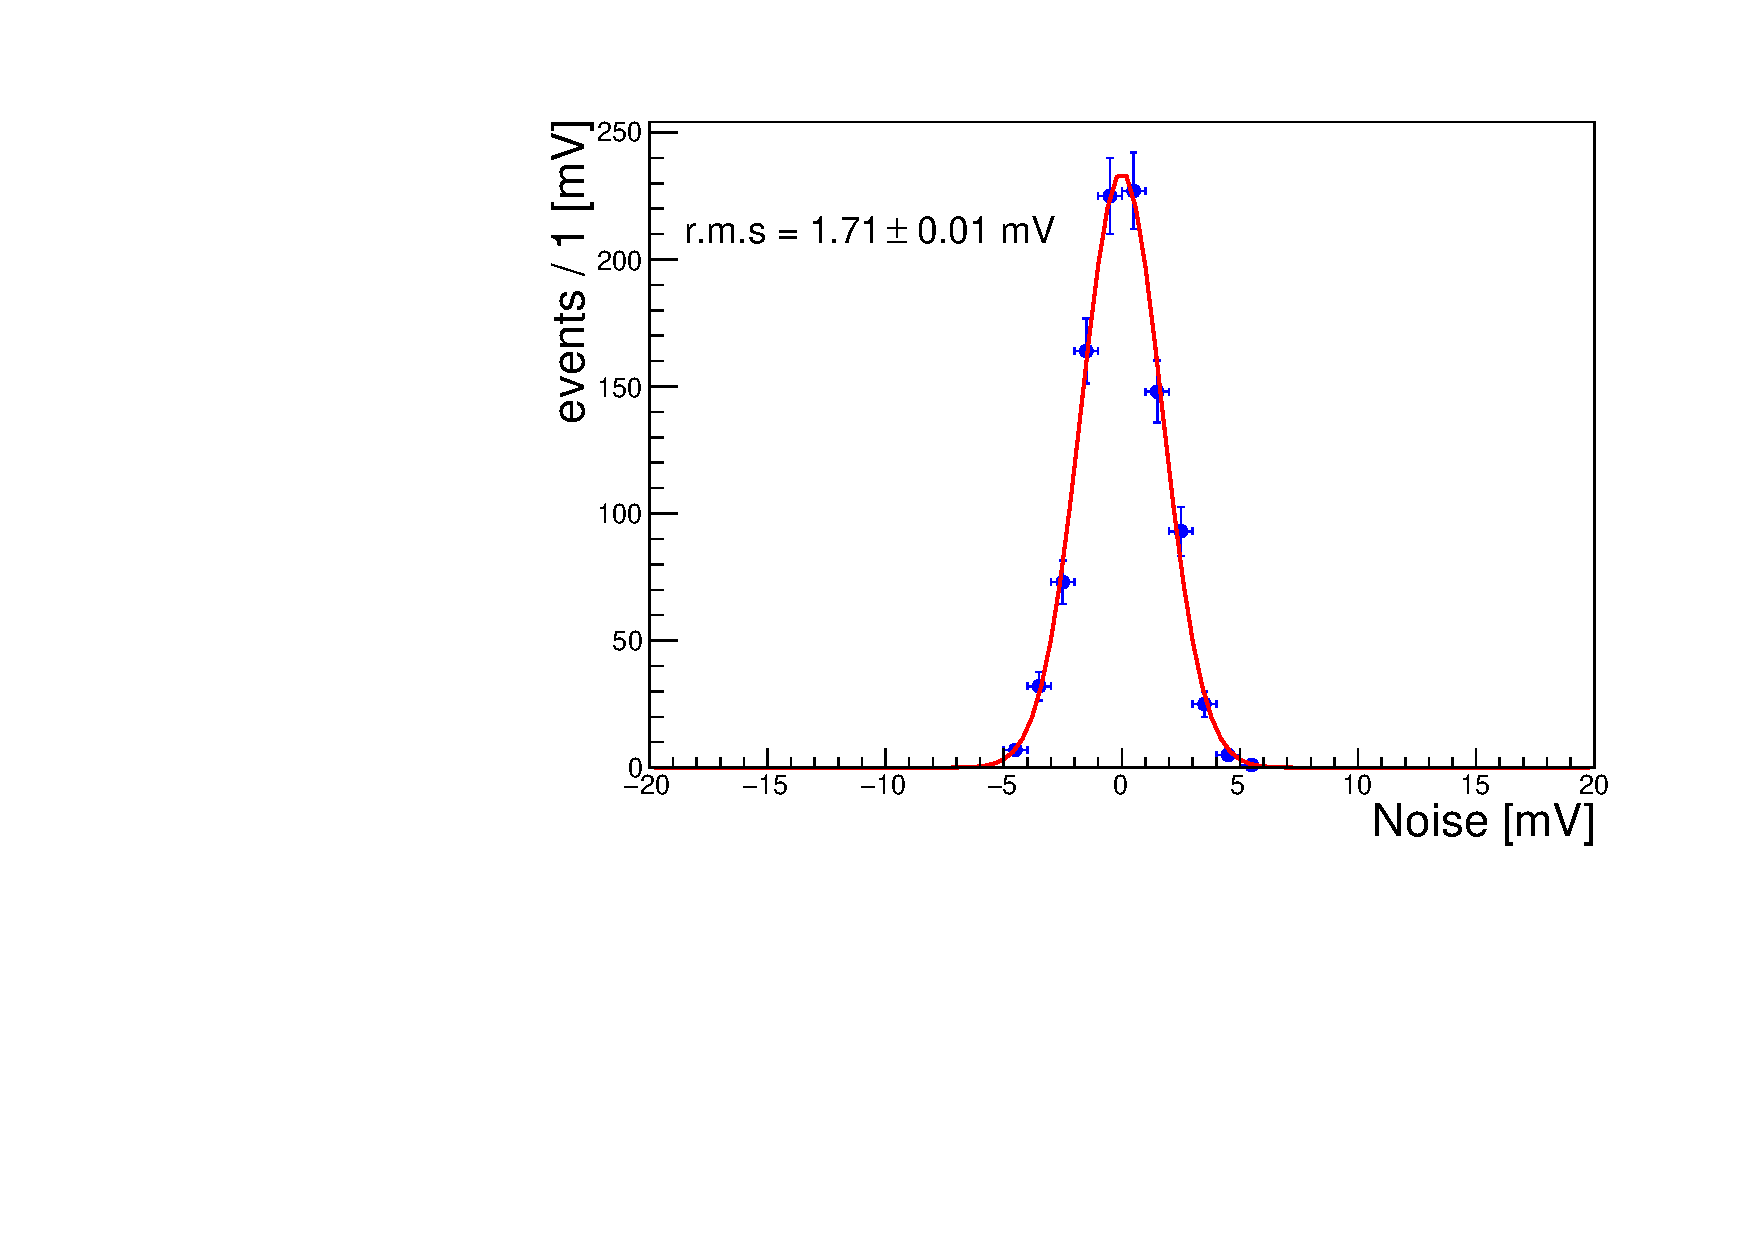
\includegraphics[width=0.48\textwidth]{figs/noise_plot_snr30.pdf}
  \caption{(Left) Amplitude distribution after the FEE. A Landau fit is performed to obtain the MPV.
  (Right) Amplitude distribution at a fixed sample of noise-only waveforms. A gaussian fit performed to obtain the r.m.s.
  Both figures correspond to a pre-radiation sensor using a shaping time (ST) of 1~\si{ns} and a SNR of 30.}
  \label{fig:amp_and_noise}
\end{figure}

\begin{figure}[htbp]
\centering
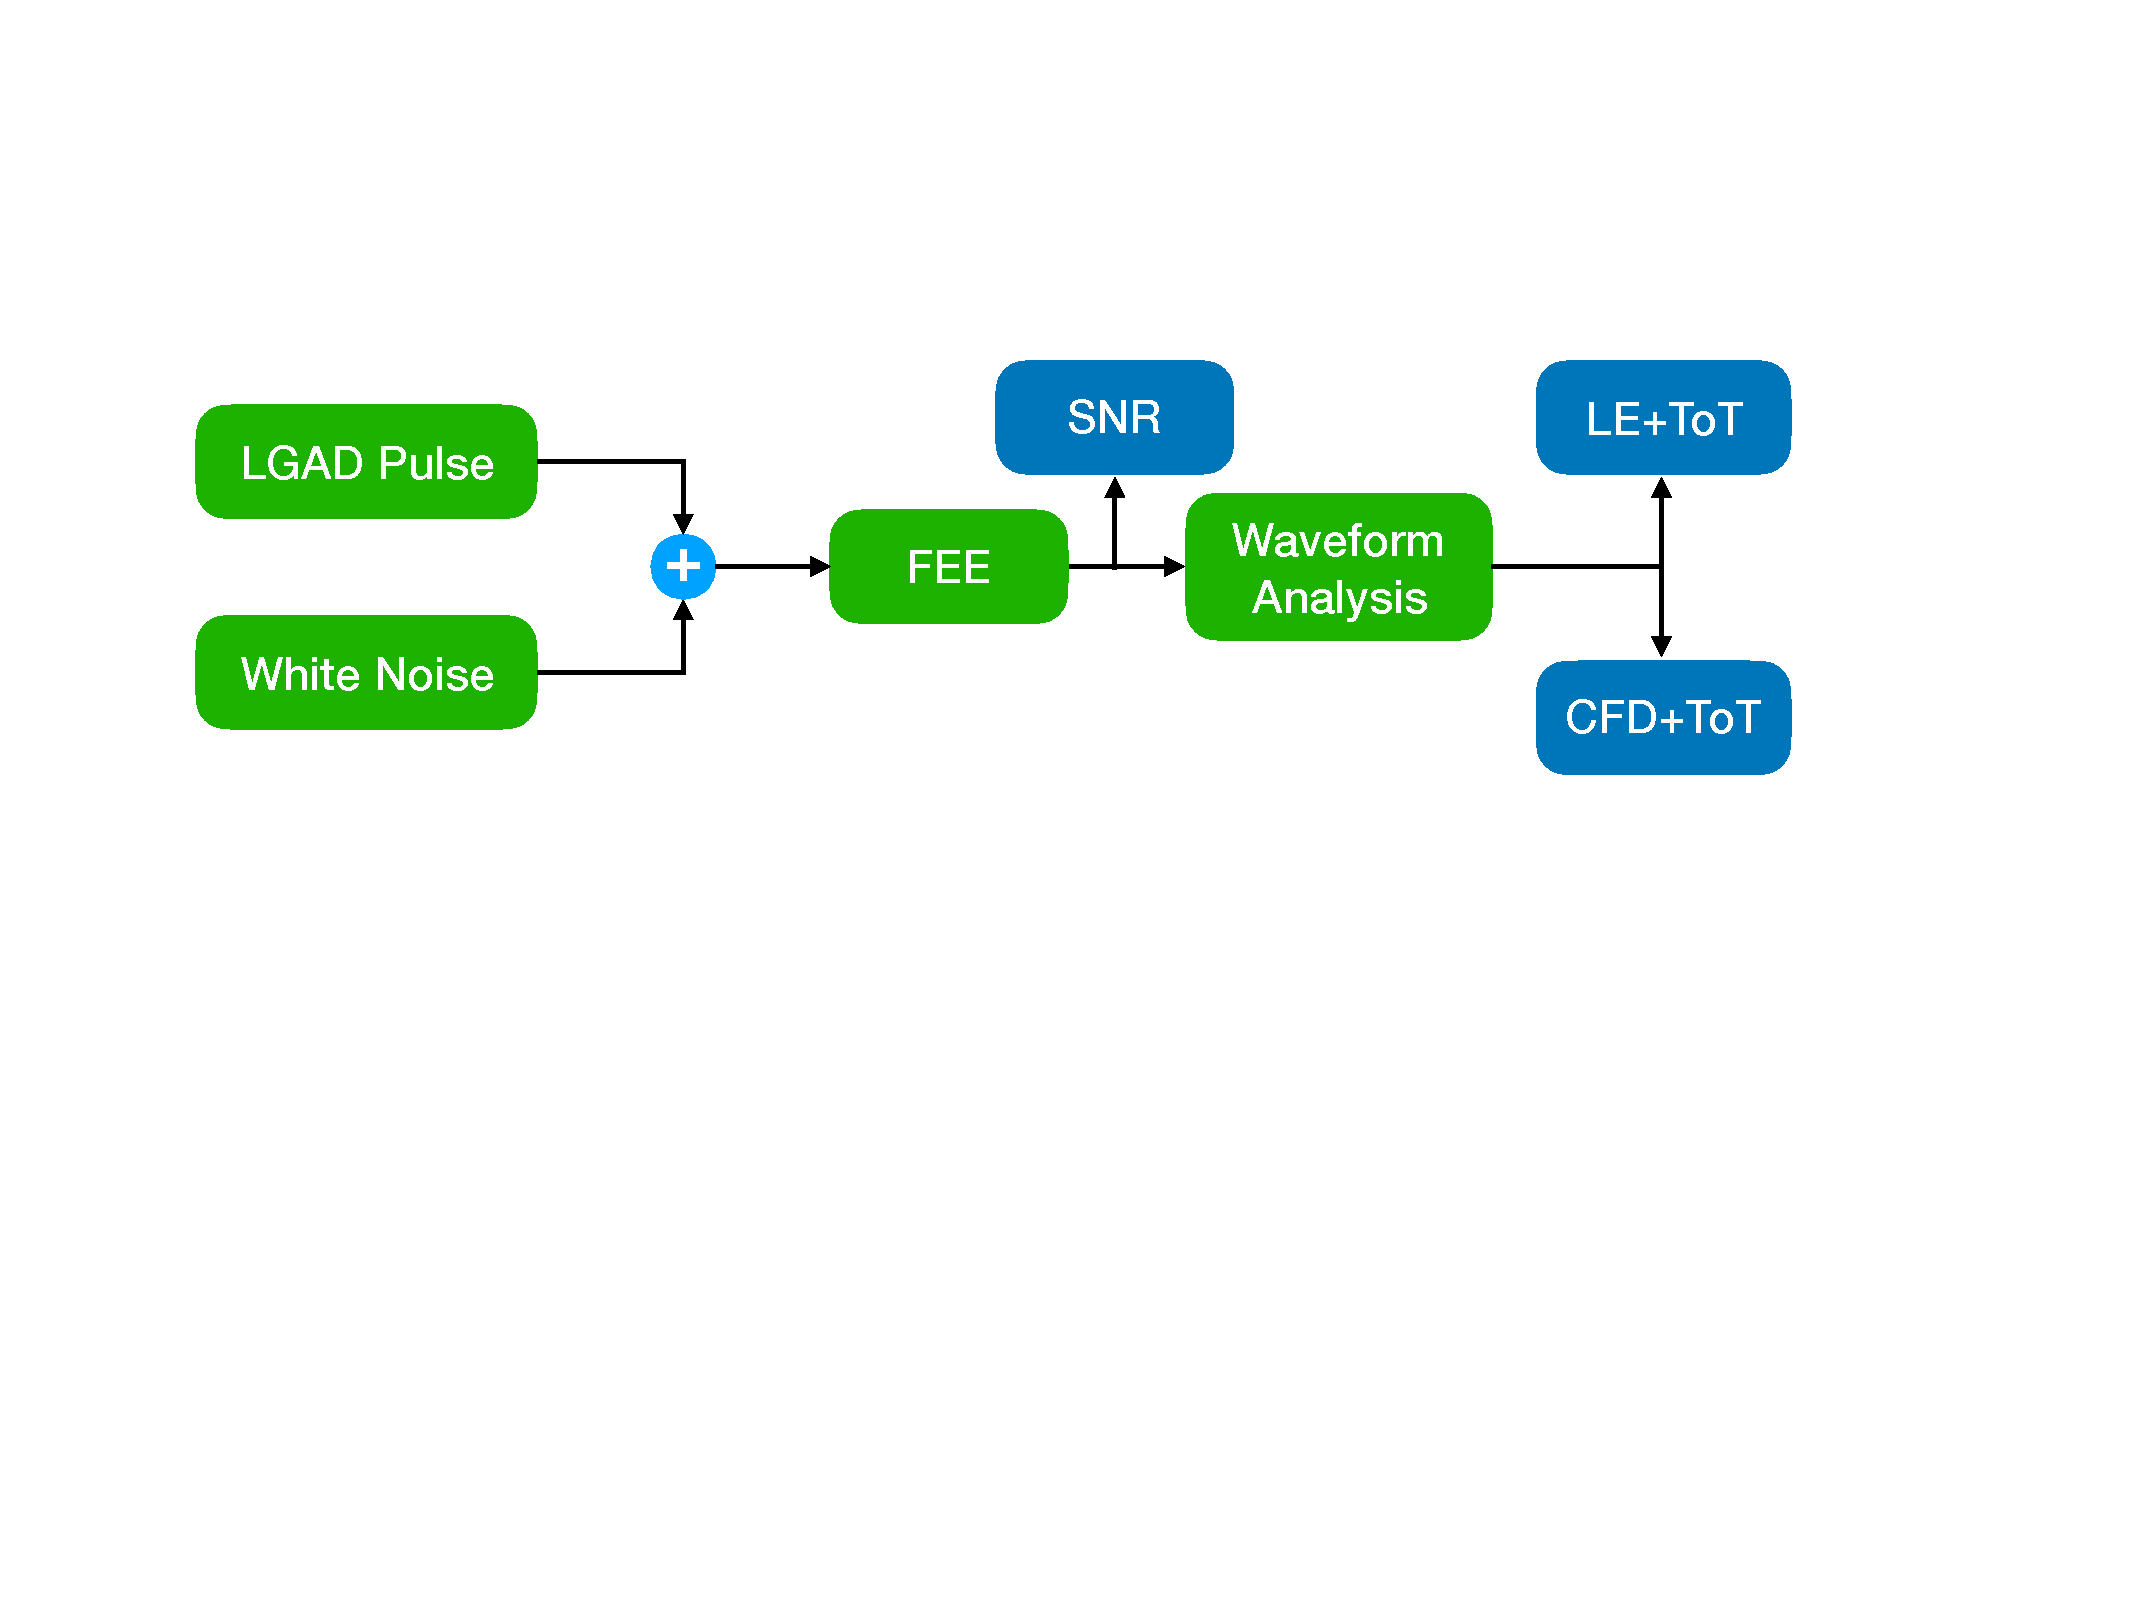
\includegraphics[width=0.75\textwidth]{figs/lgad_simulation_diagram.pdf}
\caption{A schematic diagram of the simulation. Each simulation configurable
	block is shown in green. The most relevant outputs of the simulation are shown
	in blue.} \label{fig:simulation_diagram}
\end{figure}


%\subsection{LGAD pulse library and simulation}
%\label{sub_sec:lgad_pulse_library}
%e need to ask Nicolo to send us a paragrah for the Weightfield2 (WF2)

\subsection{Front-end electronics and noise injection}
\label{sub_sec:fee_simulation_and_noise} The front-end simulation combines
analytical and numerical calculations. We implement two independent
paths of simulations, one based on the time domain and the other on the Laplace domain.
Both simulation use the unprocessed WF2 LGAD pulses as input (see Fig~\ref{fig:lgad_current}).
 The results of the two simulations are in agreement within statistical uncertainties and provide a
cross check of the results. Sections~\ref{sec:fee}
and~\ref{sec:noise_simulation} describe the details of the implementation of the
front-end and noise simulation. 

\subsubsection{Front-end simulation}\label{sec:fee}
The front-end simulation is based on a single amplification stage. 
The FEE is a second order low-pass filter with transfer function ($H(S)$)
and impulse response ($h(t)$) given by equations~\ref{eq:filter_tf} and~\ref{eq:filter_ir}, respectively.
It realizes a $\mathrm{CR-RC}^{3}$-type filter~\cite{}.

 \begin{tabularx}{\textwidth}{XX}
 \begin{equation}\label{eq:filter_tf}
   H(S) = \frac{\frac{1}{\tau_{s}^{2}}}{(S+1/\tau_{s})^{2}}
 \end{equation}
     &
 \begin{equation}\label{eq:filter_ir}
     h(t) = \frac{t}{\tau_s^2}e^{-t/\tau_{s}}
 \end{equation}
 \end{tabularx}\par
%Si: I don't like this tabular way of writing the two equations much...I suggest you just make it two equations in two lines.


The output pulse of the FEE is the convolution (in time domain) of the
unprocessed LGAD signal pulse from WF2 and the FEE impulse response function,
given in Eq.~\ref{eq:filter_ir}. The sampling period for the pulses and the
convolution is 10~\si{ps}, this choice is used throughout the
simulation. As stated above we focus the study on the BW of the FEE and to that
end we scan the $\tau_{s}$ parameter in Eq.~\ref{eq:filter_ir} in the following
set:\{0.5, 1, 2, 4\}~\si{ns}. This parameter is hereafter referred to as shaping
time (ST). Figure~\ref{fig:ir_and_lgad} (left) shows the comparison of the
impulse response and a characteristic example LGAD response for a ST of 1~\si{ns} while
Figure~\ref{fig:ir_and_lgad} (right) shows the LGAD response for all STs
studied. We observe that the LGAD response peaks later with respect to the
impulse response,  and that pulse slew rate is decreased in the first nanosecond
of the pulse. As expected, we also observe that the pulse risetime, defined as
the time required for the signal to rise from 10\% to 90\% of its
amplitude,  increases with the ST. Table~\ref{tab:risetime} summarizes the risetime
for the set of ST studied. 

\begin{figure}[htbp]
  \centering
  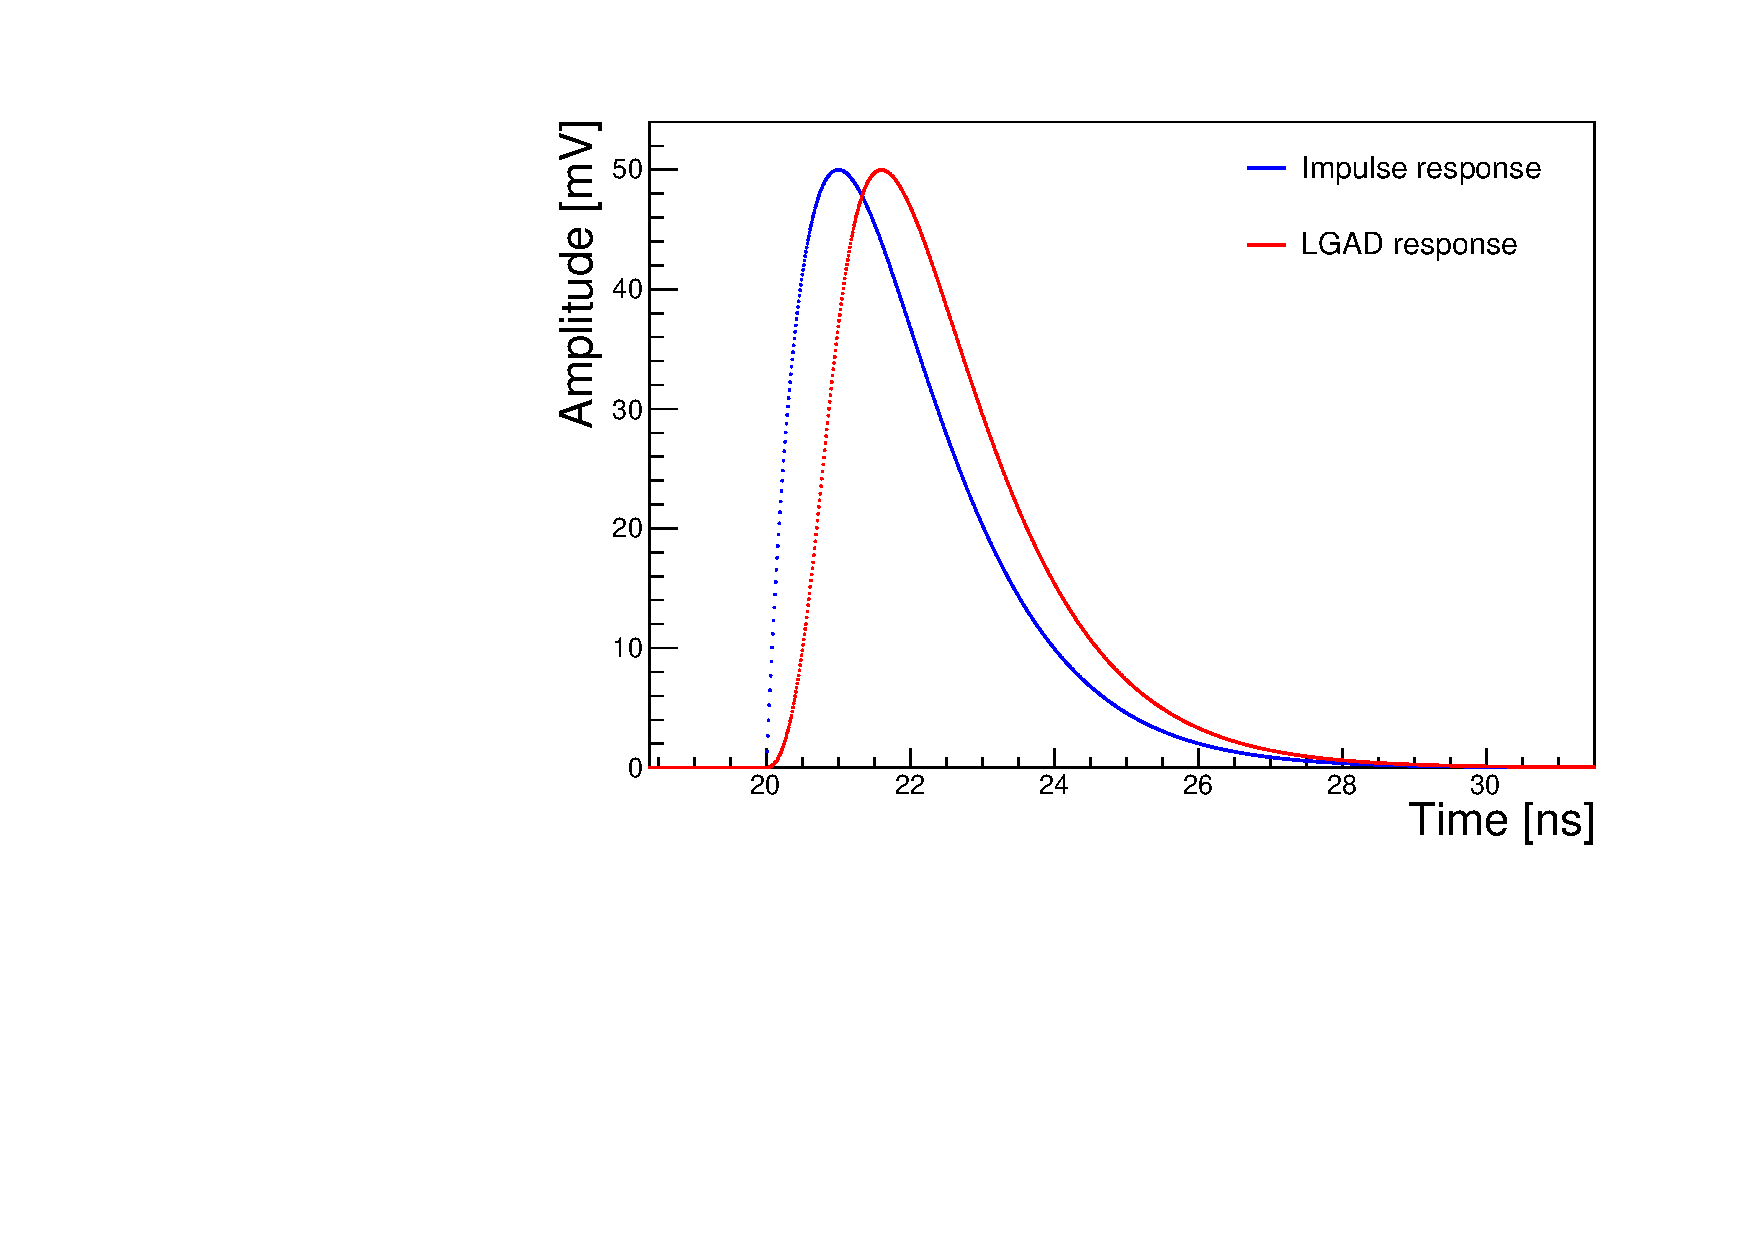
\includegraphics[width=0.48\textwidth]{figs/impulse_vs_lgad_response_1ns_shaping.pdf} \hfill
  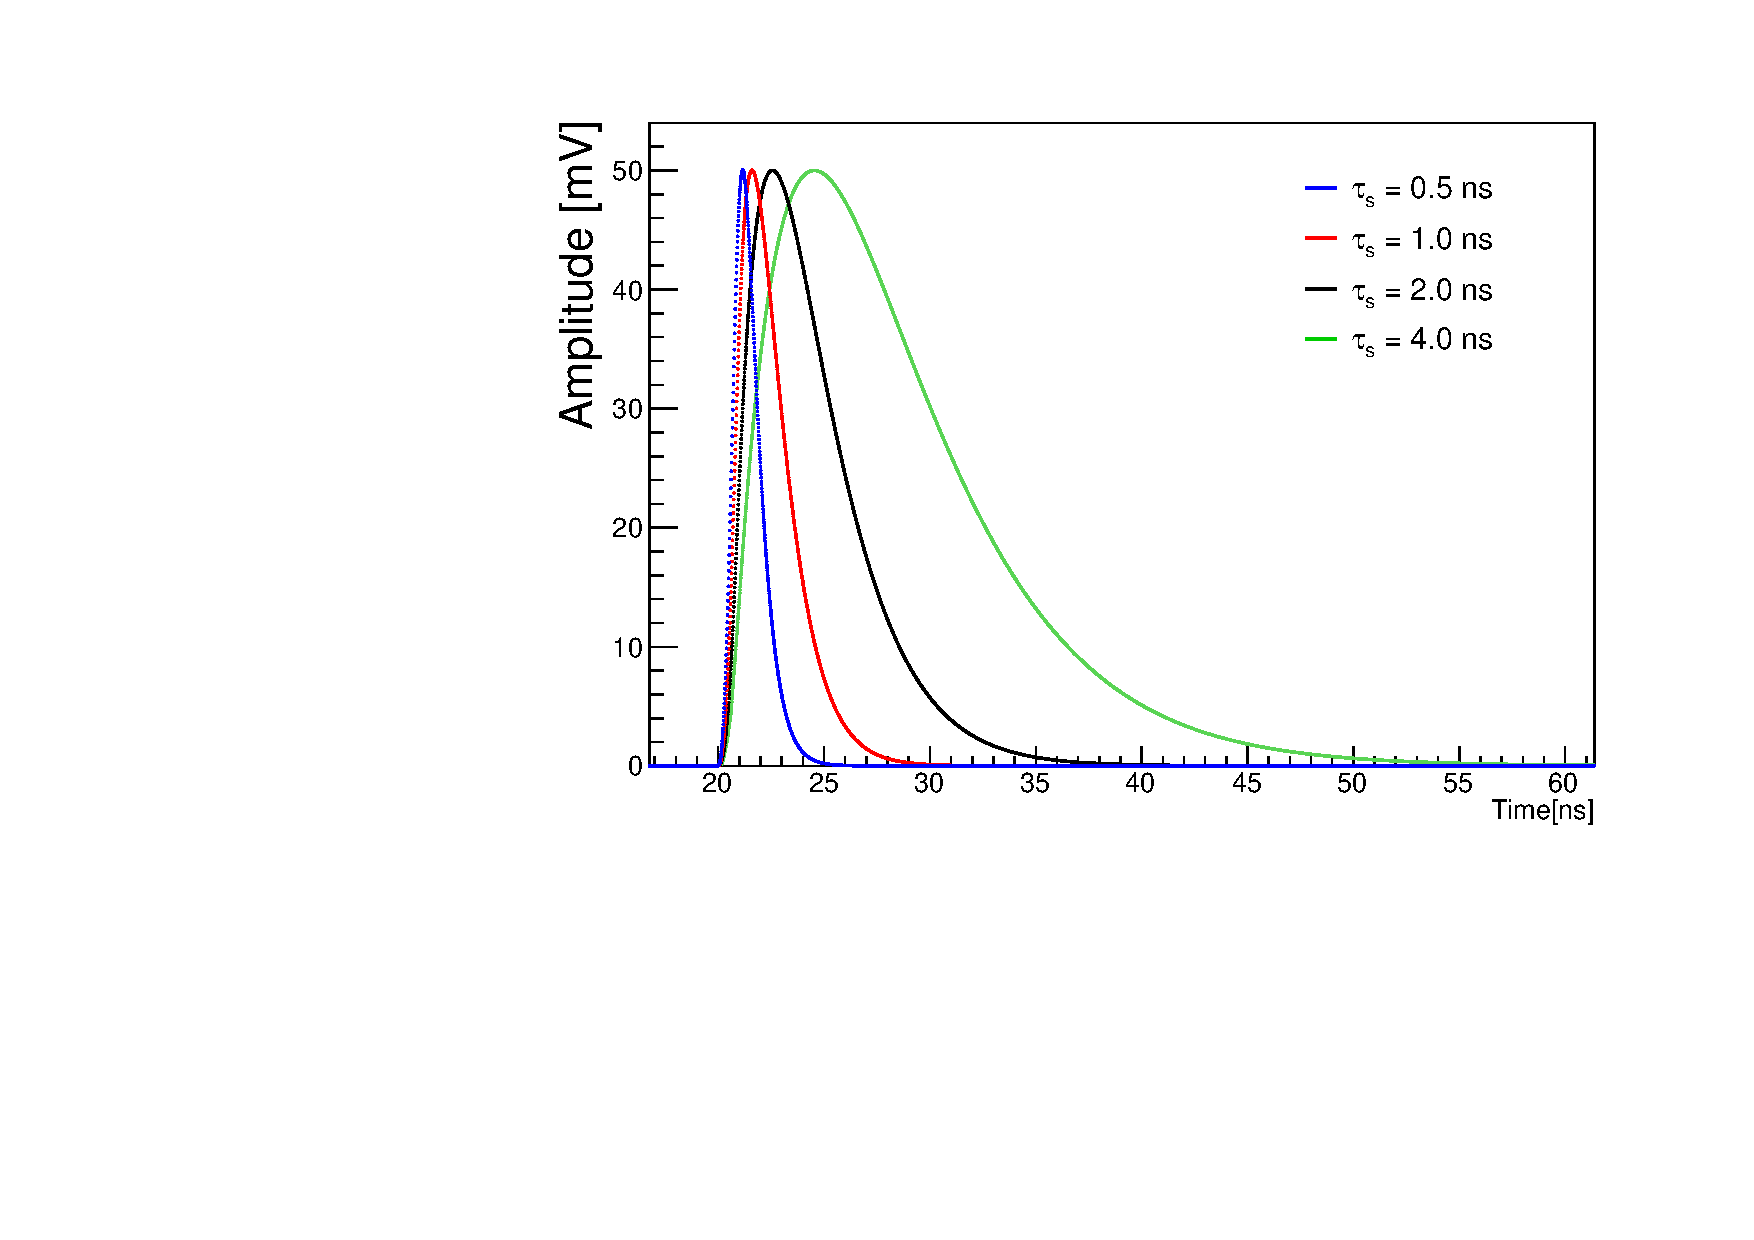
\includegraphics[width=0.48\textwidth]{figs/lgad_all_shaping_time_noiseless.pdf}
  \caption{(Left) Comparison of impulse and characteristic LGAD responses for the a shaping time (ST) of 1~\si{ns}.
  (Right) LGAD response for the four shaping times studied: \{0.5, 1, 2, 4\}~\si{ns}. All pulses have been normalized
  to achive a peak amplitude of 50~\si{mV}. }
  \label{fig:ir_and_lgad}
\end{figure}


\begin{table}\label{tab:risetime}
  \begin{center}
    \begin{tabular}{c|cccc}
    %\multicolumn{1}{c}{}& \multicolumn{4}{c}{Risetime (10-90\%) (ps)} \\
    %\multicolumn{1}{c}{}& \multicolumn{3}{c}{$\mathrm{(RC)}^{2}$ Constant Fraction}\\ \hline
    ST (ns) & 0.5  & 1.0 & 2.0 & 4.0 \\\hline
    Risetime (ns) & $0.67\pm 0.02$ & $0.86\pm 0.02$ & $1.36\pm 0.02$ & $2.48\pm 0.02$ \\
    \end{tabular}
    \caption{Measured risetime for all shaping times studied: \{0.5, 1, 2, 4\}~\si{ns}. The uncertainty is the r.m.s of the
    risetime distribution.}
  \end{center}
 \end{table}

%Si: What are the uncertainties ``xx''?



\subsubsection{Noise injection}\label{sec:noise_simulation}
Gaussian white noise is simulated by sampling every 10~\si{ps}~\cite{Radeka}. Each
sampled time is assigned a random amplitude which is drawn from a gaussian distribution with zero mean and width corresponding to the SNR
under study. Based on Parseval's theorem, the noise amplitude needs to be adjusted depending
on the ST of the FEE for a given sampling rate. The left panel of Figure~\ref{fig:noise} shows the gaussian white noise before and after a filter with 
1~\si{ns} shaping time. We checked that the average noise power spectrum is flat in the frequency domain up to
at least 10 GHz. We observe the expected $\sqrt(\mathrm{BW})$ scaling of the noise after
 the FEE for all the STs under study. The right panel of Figure~\ref{fig:noise} shows an example output of the
FEE block, with a 1~\si{ns} ST, for a pre-irradiated LGAD pulse after noise has been injected. The injected noise is
such that the SNR is 30. 

\begin{figure}[htbp]
  \centering
  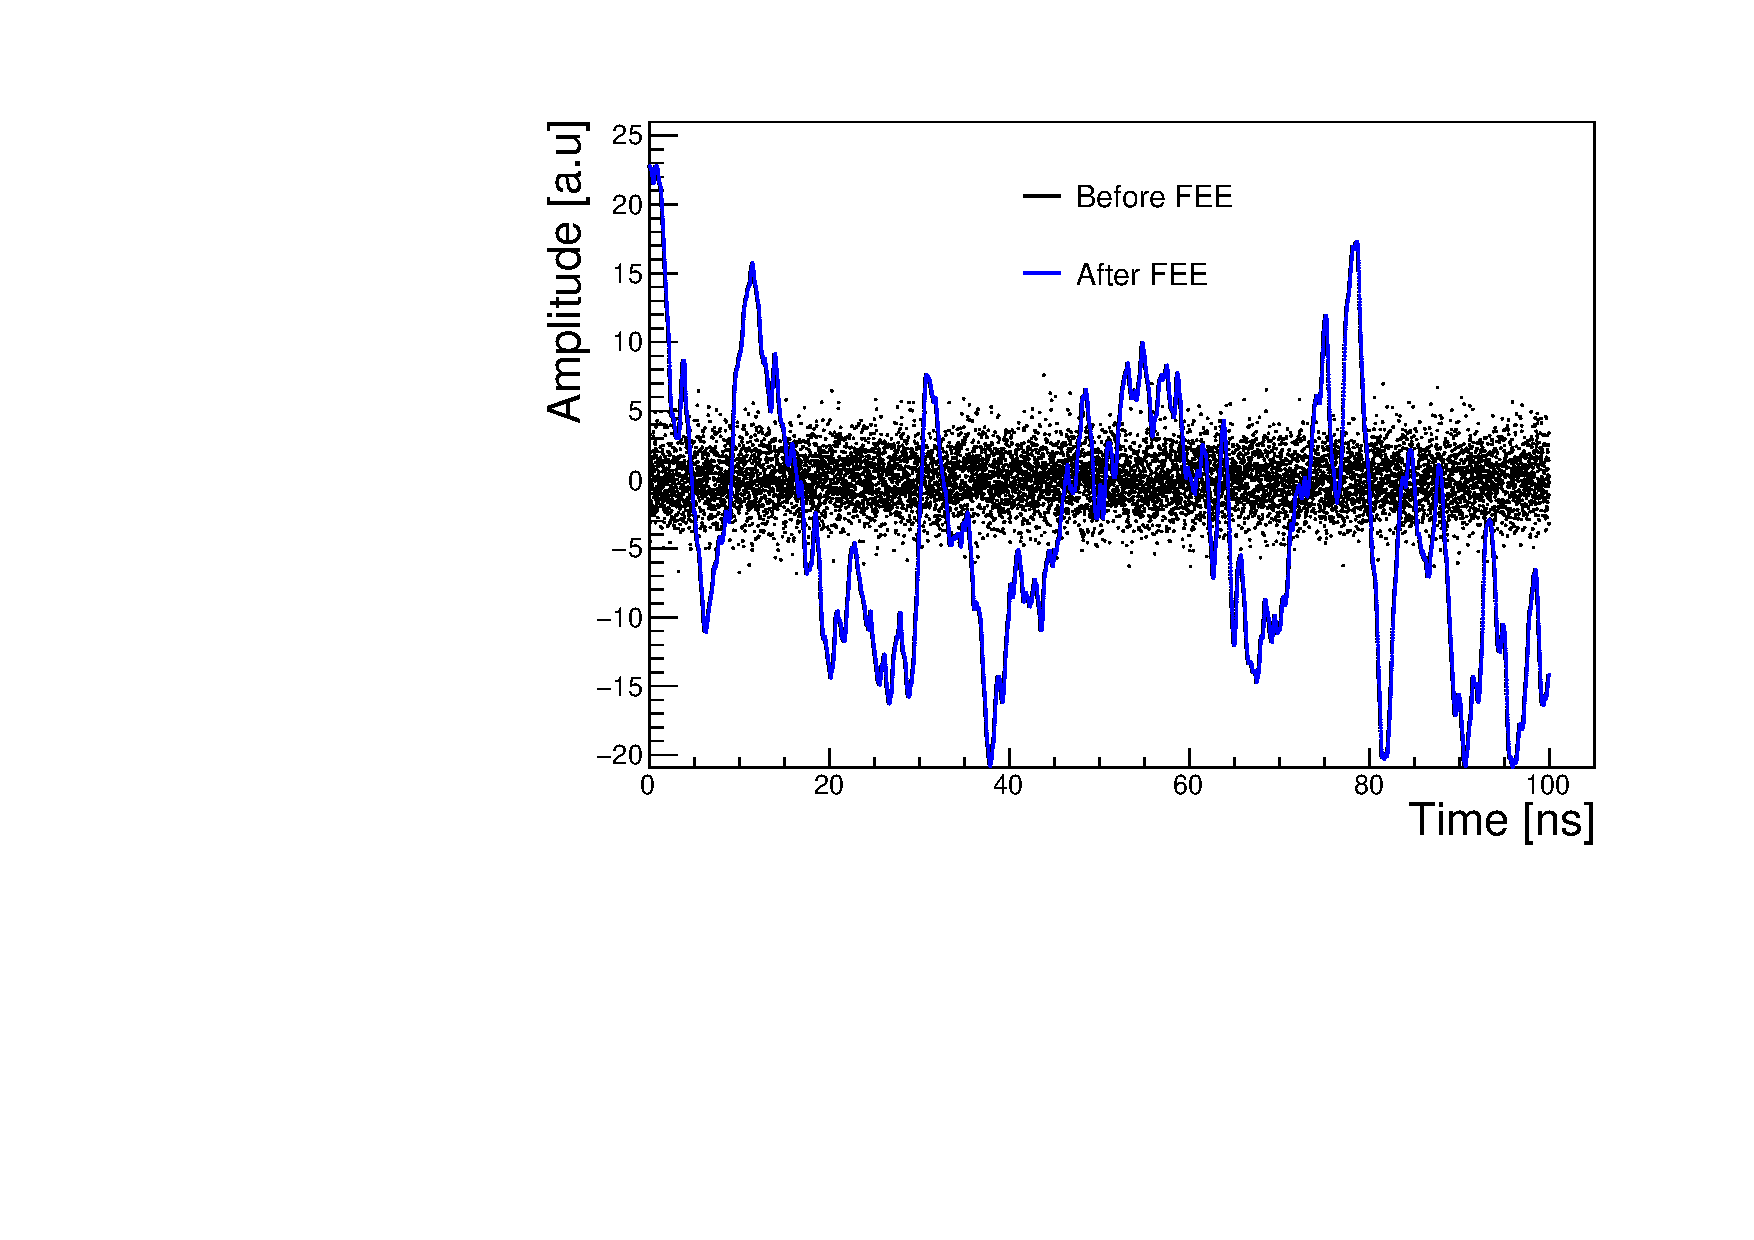
\includegraphics[width=0.48\textwidth]{figs/noise_vs_shaped_noise.pdf} \hfill
  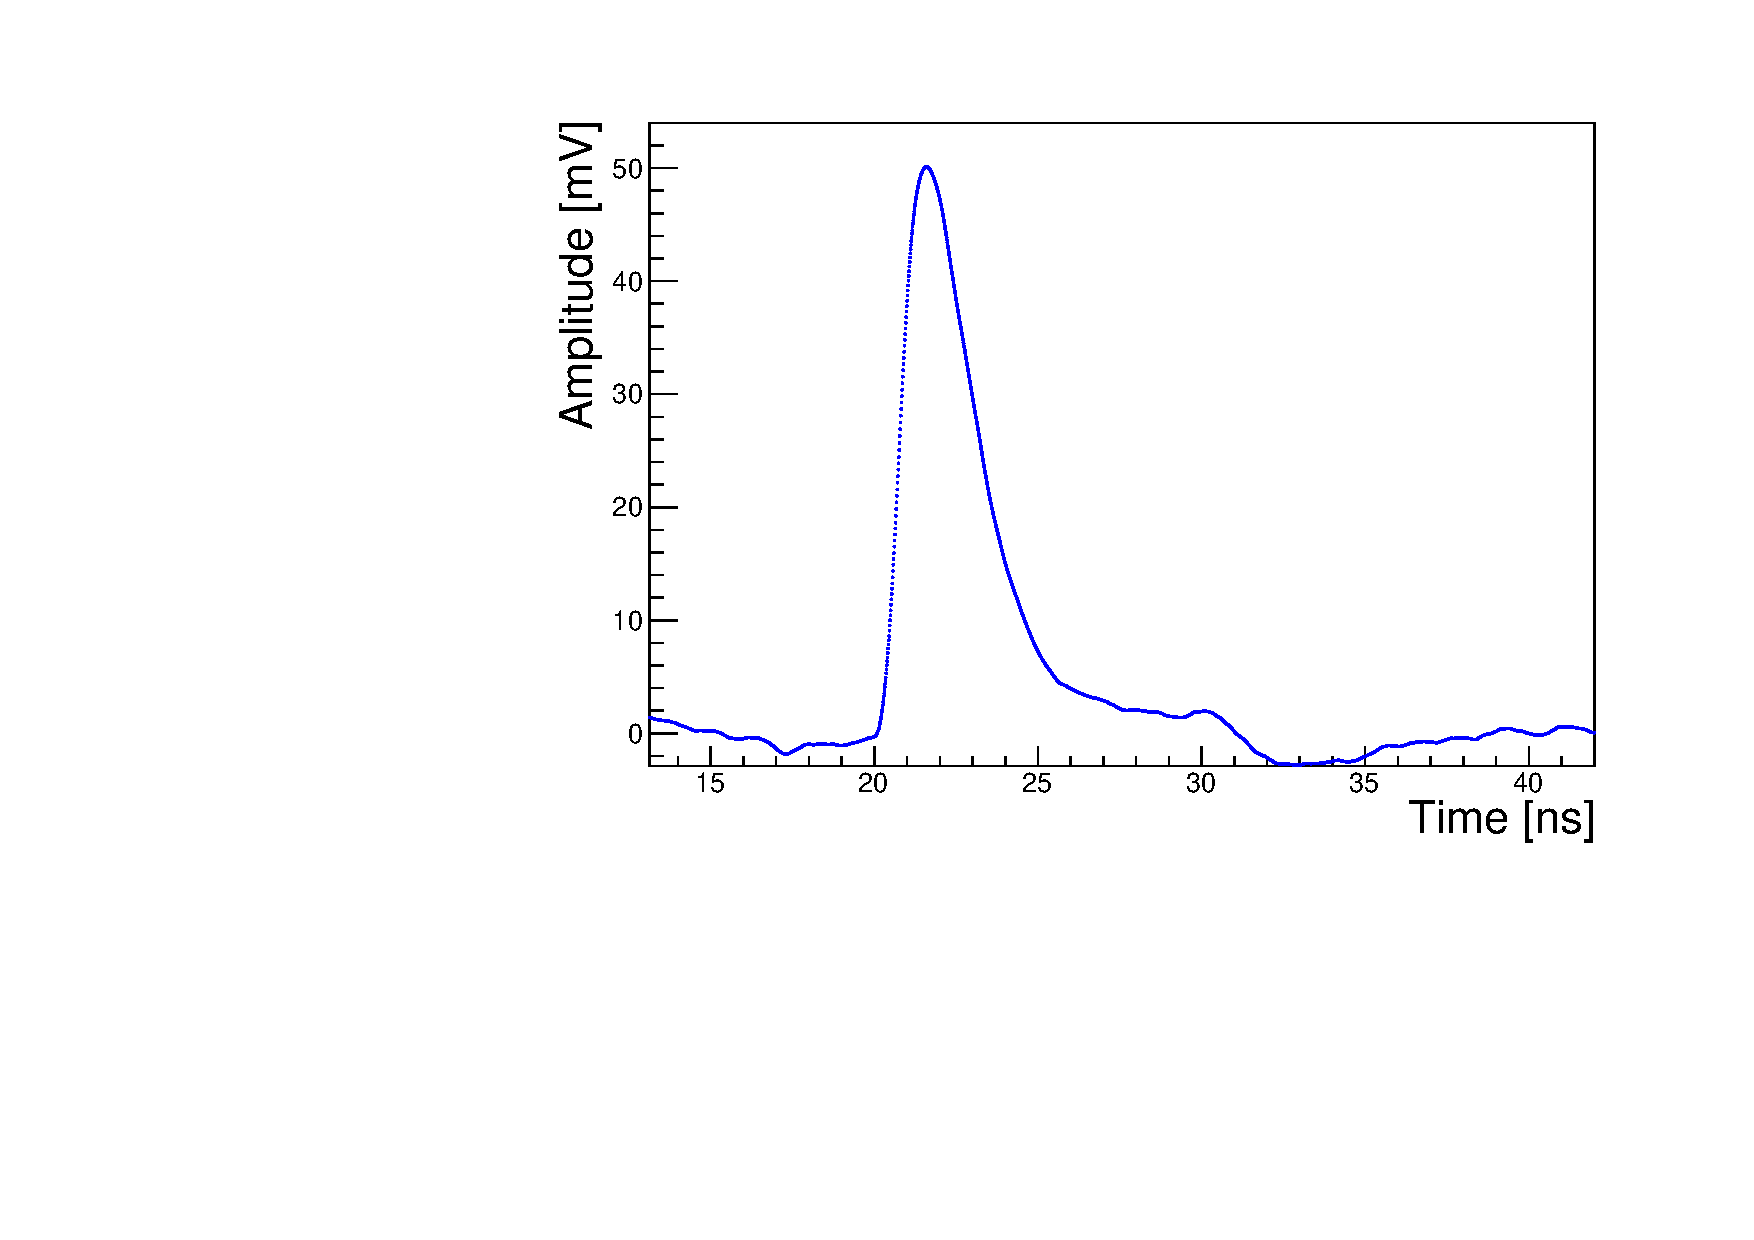
\includegraphics[width=0.48\textwidth]{figs/lgad_pre_rad_st_1ns_snr_30.pdf}
  \caption{(Left) Comparison of gaussian white noise before and after the FEE, legend is shown in plot.
  (Right) Example pulse at the output of the FEE block with a SNR of 30. Both figure use a shaping time (ST) of 1~\si{ns}.}
  \label{fig:noise}
\end{figure}

\section{Timing Reconstruction and Analysis}\label{sec:timing_and_analysis}
The time reconstruction is based on waveform analysis. We generate an ensemble of 1000 pulses for each 
simulated LGAD waveform sampled every 10 ps.
Each pulse is interpolated using the Whittaker-Shannon formula~\cite{whittaker_1915,shannon_1935}
\begin{equation}\label{eq:WS}
  f(t) = \sum f(k\mathrm{T})\frac{sin(\pi(t/\mathrm{T} - k))}{\pi(t/\mathrm{T} - k)}.
\end{equation}

Where f is pulse we want to interpolate, $t$ is the continuous time variable,
$k =0, \pm 1, \pm 2, ...$, and T is the sampling time (10~\si{ps}).
Using the interpolated pulse we assign a timestamp by finding when
a given voltage threshold has been crossed. The threshold can be a constant value (LE) or a constant fraction
 of the pulse height (CF).
In the case of the CFD we also simulate more realistic implementations: {\color{red}split-and-delay as well as as second order RC filter (Greg, please check naming)}.
 More details about the algorithms are given in Sec.~\ref{sec:le_and_cfd}. The time resolution is estimated by the width parameter
of a gaussian fit to the timestamps obtained for a particular theshold. We apply a time-walk correction based on the
time-over-threshold of the pulse. We note that this correction has a large improvement on the time resolution measured
using the LE algorithm while the CF algorithm is mostly insentive to this correction, as seen in Fig.~\ref{fig:time_resolution_scan}.
Details about this correction are covered in Sec.~\ref{sec:tw_and_tot}.
%The timestamps are measured with a 20~\si{ps} binning while the time-over-threshold is measured with a 100~\si{ps} binning in order to simulate the effect of time quantization.
We scan the LE and CF threshold such that we find the one with the best time resolution.

\subsection{Leading edge and constant fraction discriminators}\label{sec:le_and_cfd}
The leading edge and constant fraction discriminator algorithms are \textit{ideal} in the sense that they don't simulate the effect of
electronics in a real implementation. Our approach is to sample the pulses every 10~\si{ps} and subsequently interpolate them
using the Whittaker-Shannon formula (sin(x)/x) to more accurately determine the threshold crossing. In the LE case the threshold is scanned
from 3--60~\si{mV}, while the CFD is scanned from 5--90~\% of the current pulse maximum amplitude. For each threshold we obtain two
timestamps: when the pulse first crosses the threshold ($t_{0}$) and when it crosses the second time ($t_{1}$), now in the opposite
direction. The time-over-threshold is defined as the difference of the two timestamps ($\mathrm{ToT} = t_{1} - t_{0}$). The first
timestamp, $t_{0}$, is used to determine the time resolution at given threshold. The time resolution is defined as the width of
a gaussian fit to the $t_{0}$ distribution binned with a bin-width of 20~\si{ps}. The time resolution is obtained in two cases:
before and after a time-walk correction. The time-walk correction aims to correct the known effect of time drift as a function
of the pulse height. The time-walk correction removes this time drift and ensures that the time response is flat as a function
of the pulse height. Figure~\ref{fig:time_resolution_scan} shows the time resolution as a function
of the threshold required for a pre-irradiated LGAD sensor with a ST of 1~\si{ns} and a SNR of 30.
Fig.~\ref{fig:time_res} shows a typical $t_{0}$ distribution, using the LE and CF algorithms, for the pre-irradiated
LGAD sensor after the ToT correction has been applied. The time resolution ($\sigma_{t}$) is measured to be $37.3 \pm 1.4 $
and $33.0 \pm 1.4$ for the LE and CF, respectively. Additionally, we study a more practical CFD implementation
based on the subtraction of a scaled signal from a delayed one, where the delay is achieved either using an ideal 
delay element or an RC-type low pass filter. We observe that the practical CFD implemented using an ideal delay element 
yields equivalent results as the ideal CFD to within uncertainties. The more realistic CFD implemented using 
an RC-type low pass filter yields a slightly degraded performance.

  \begin{figure}[htbp]
    \centering
    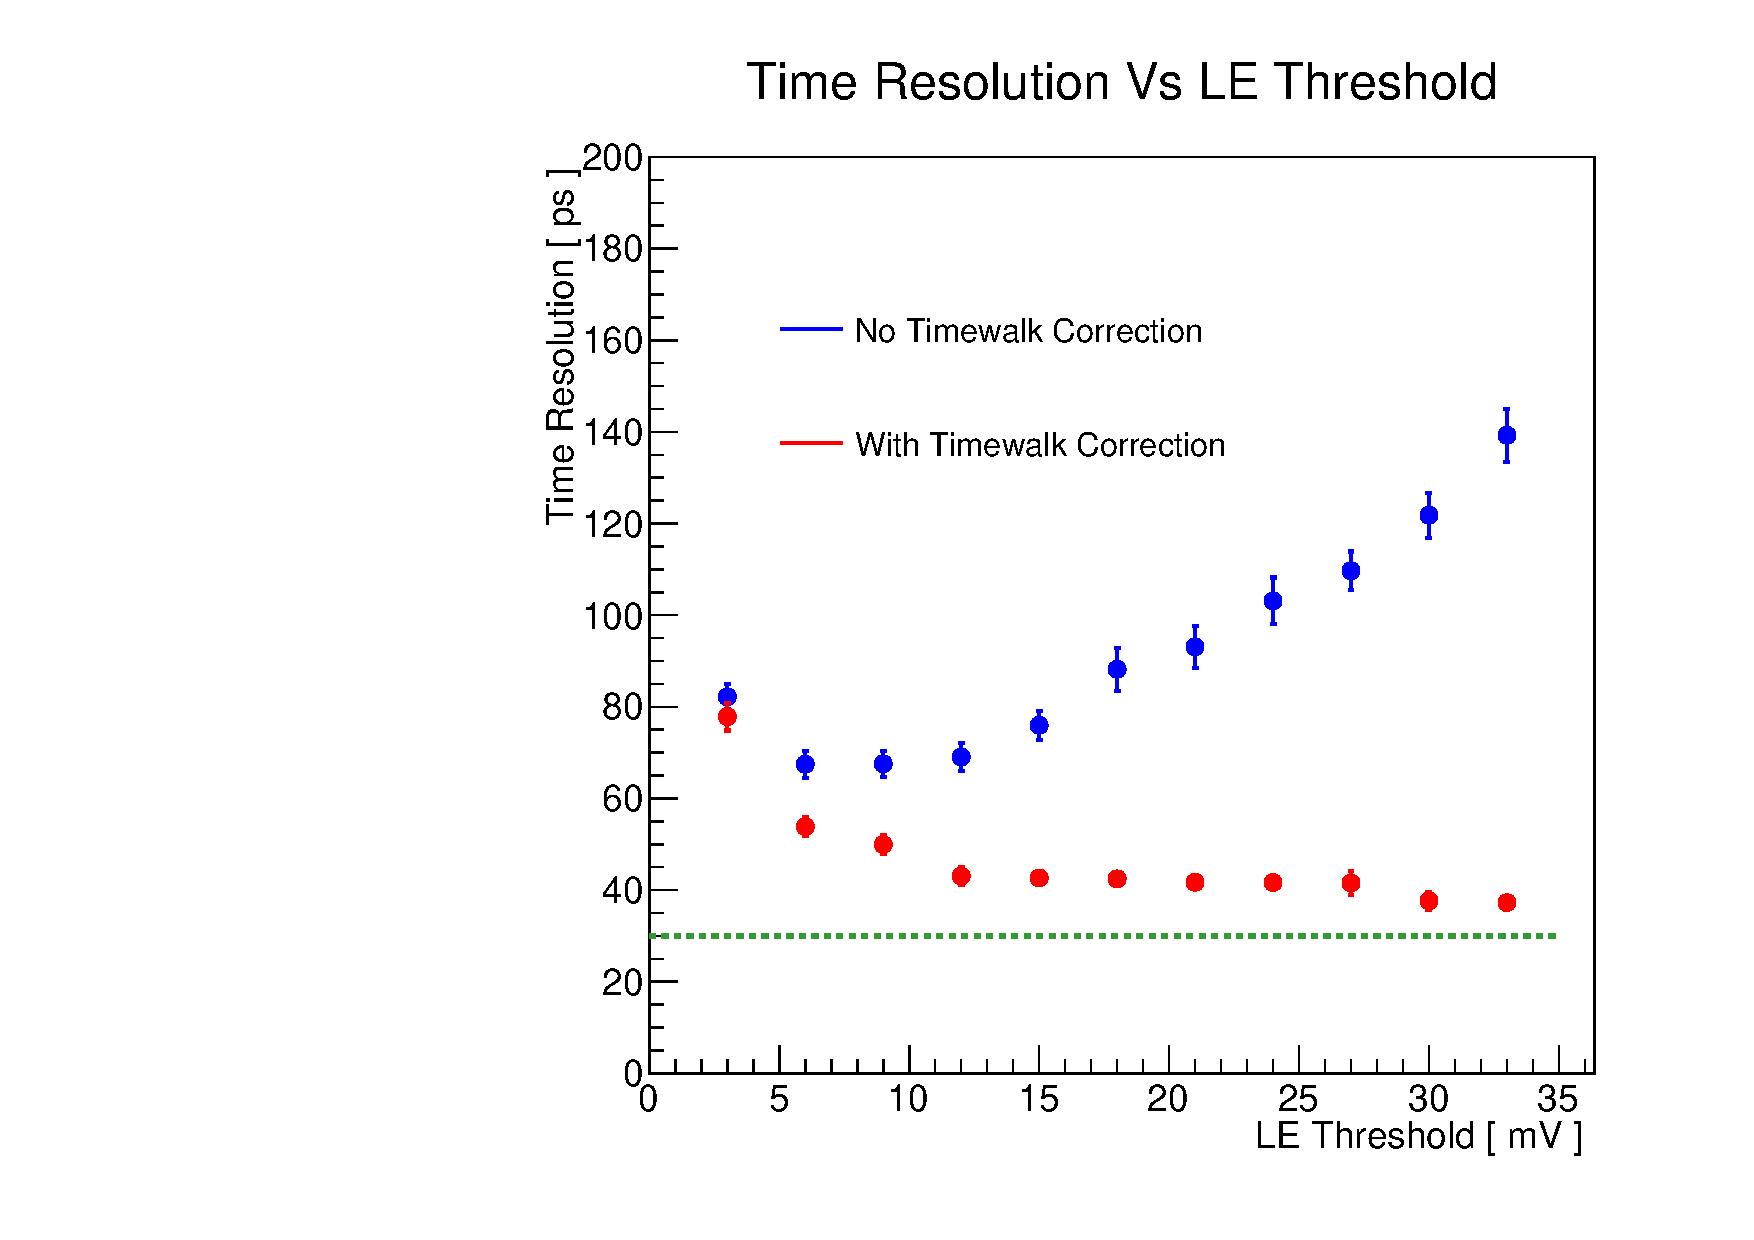
\includegraphics[width=0.48\textwidth]{figs/ShapingTime1p0_SNR30_55MicronGain15Prerad_FIXED_NOISE_FIXED_SNR_V2_converted_TimeResolutionVsThresholdToT.pdf} \hfill
    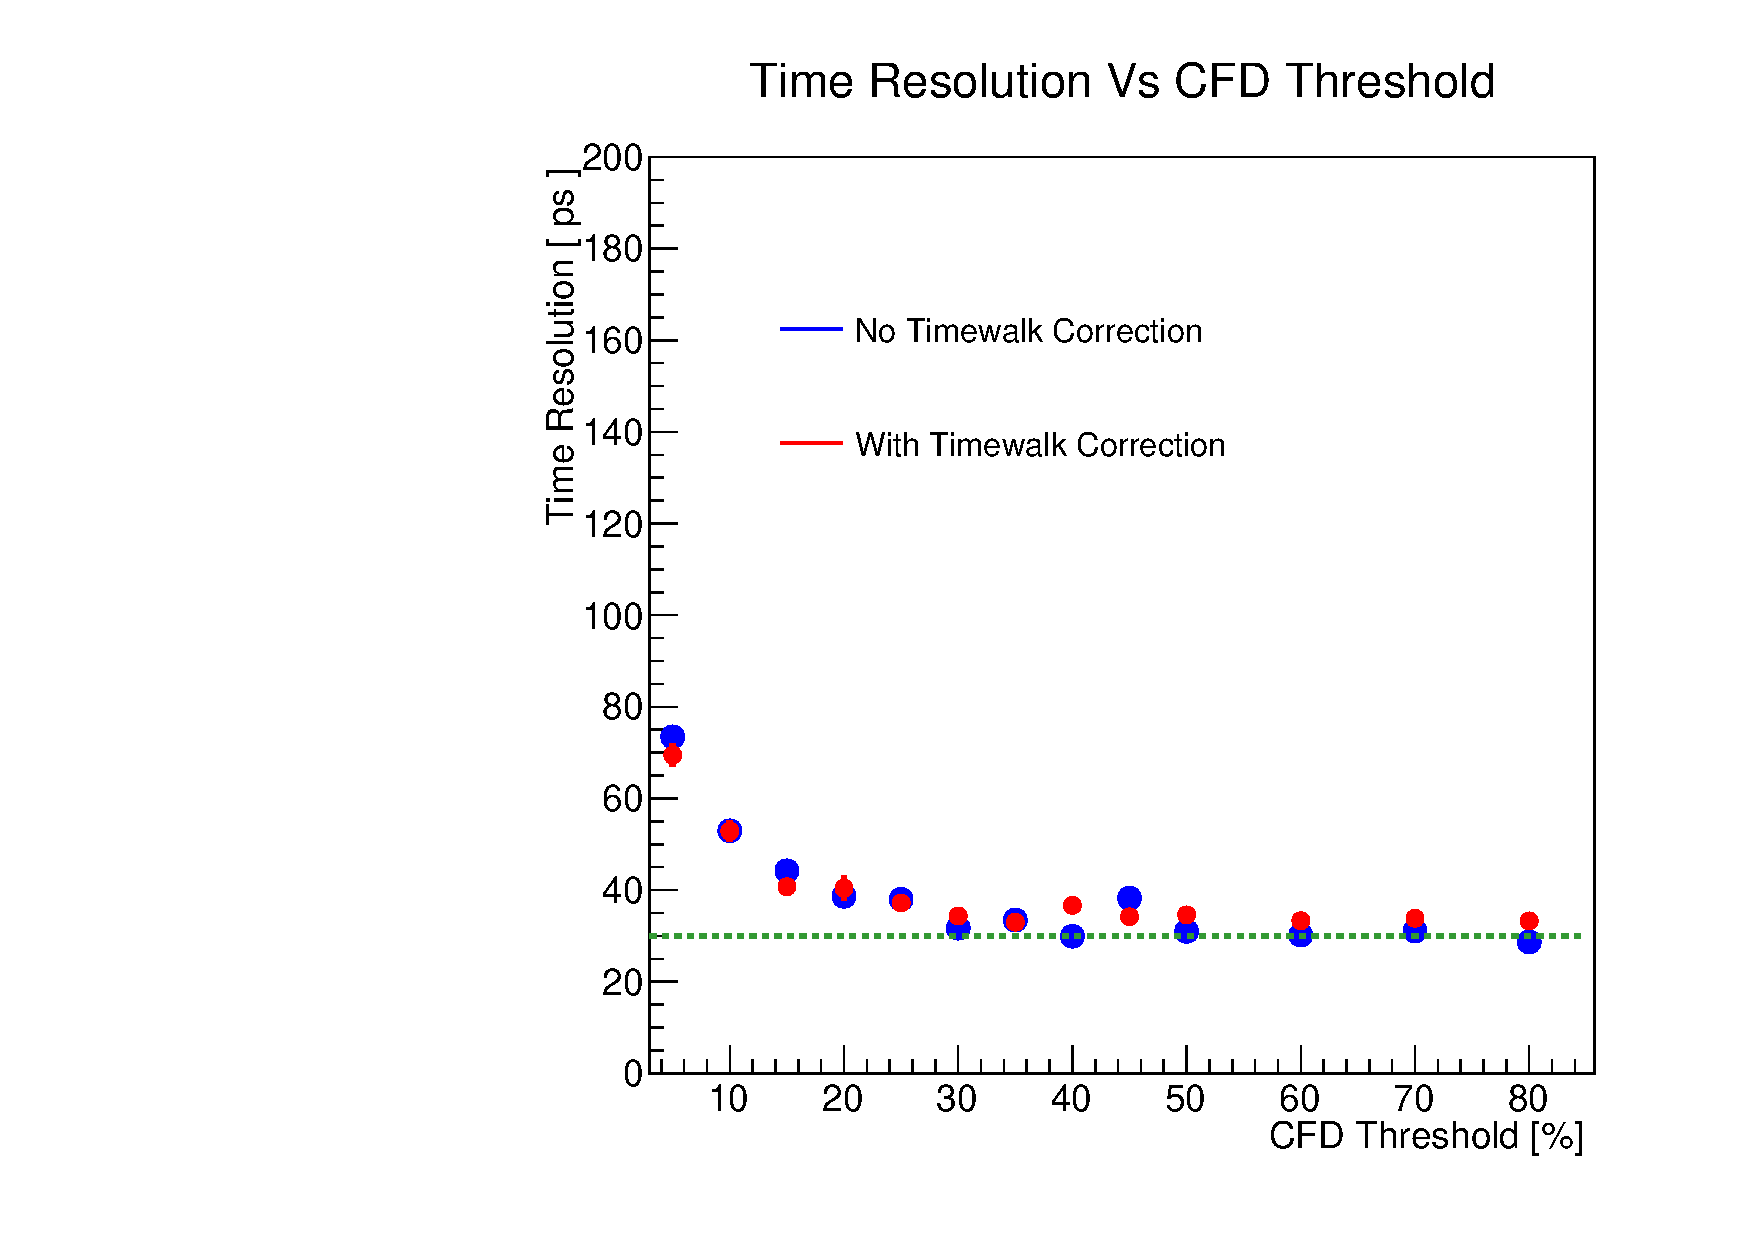
\includegraphics[width=0.48\textwidth]{figs/ShapingTime1p0_SNR30_55MicronGain15Prerad_FIXED_NOISE_FIXED_SNR_V2_converted_TimeResolutionVsThresholdCFD.pdf}
    \caption{(Left) LE time resolution as a function of threshold.
    (Right) CF time resolution as a function of threshold.
    Both figure use pre-irradiated LGAD sensor with a ST of 1 ns and a SNR of 30.}
    \label{fig:time_resolution_scan}
  \end{figure}

  \begin{figure}[htbp]
    \centering
    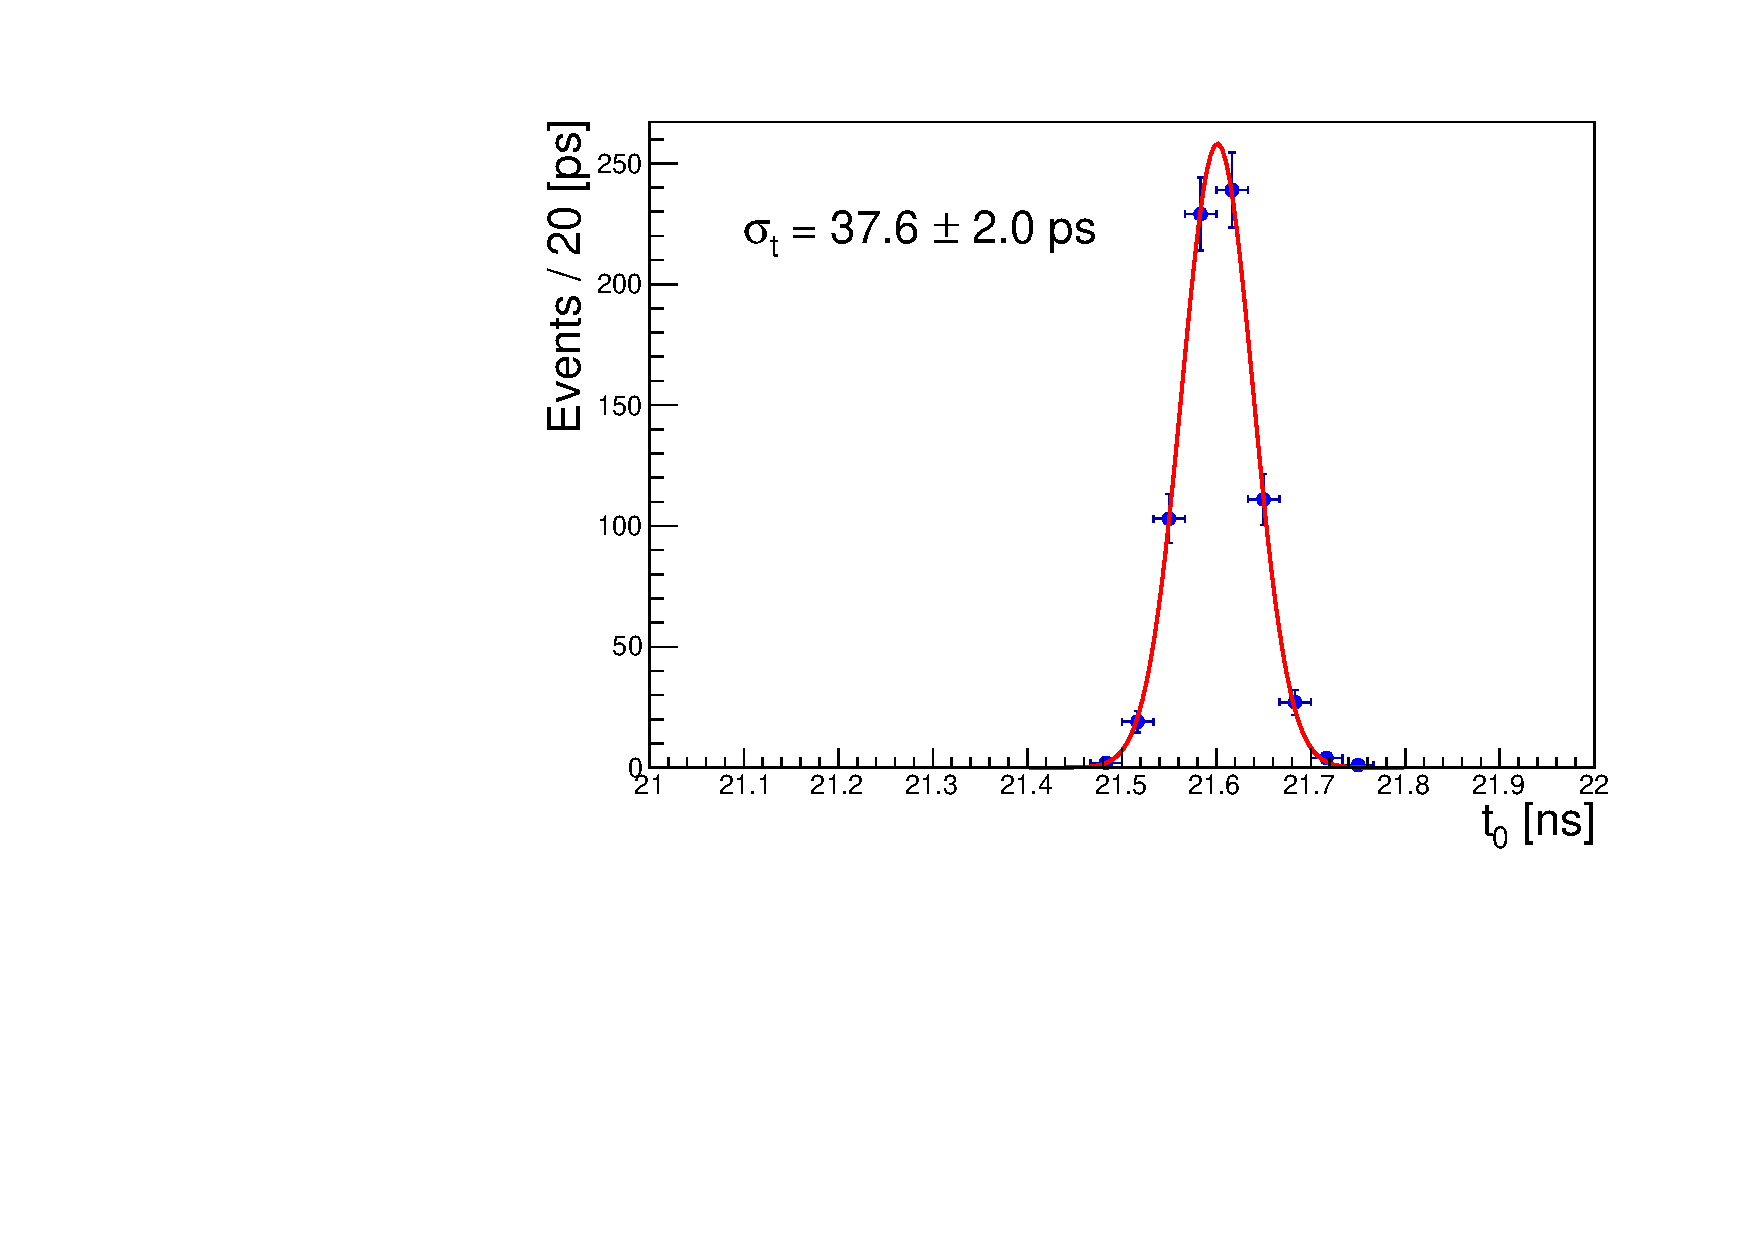
\includegraphics[width=0.48\textwidth]{figs/pre_rad_st_1ns_snr_30_le_tot_threshold_30mV.pdf} \hfill
    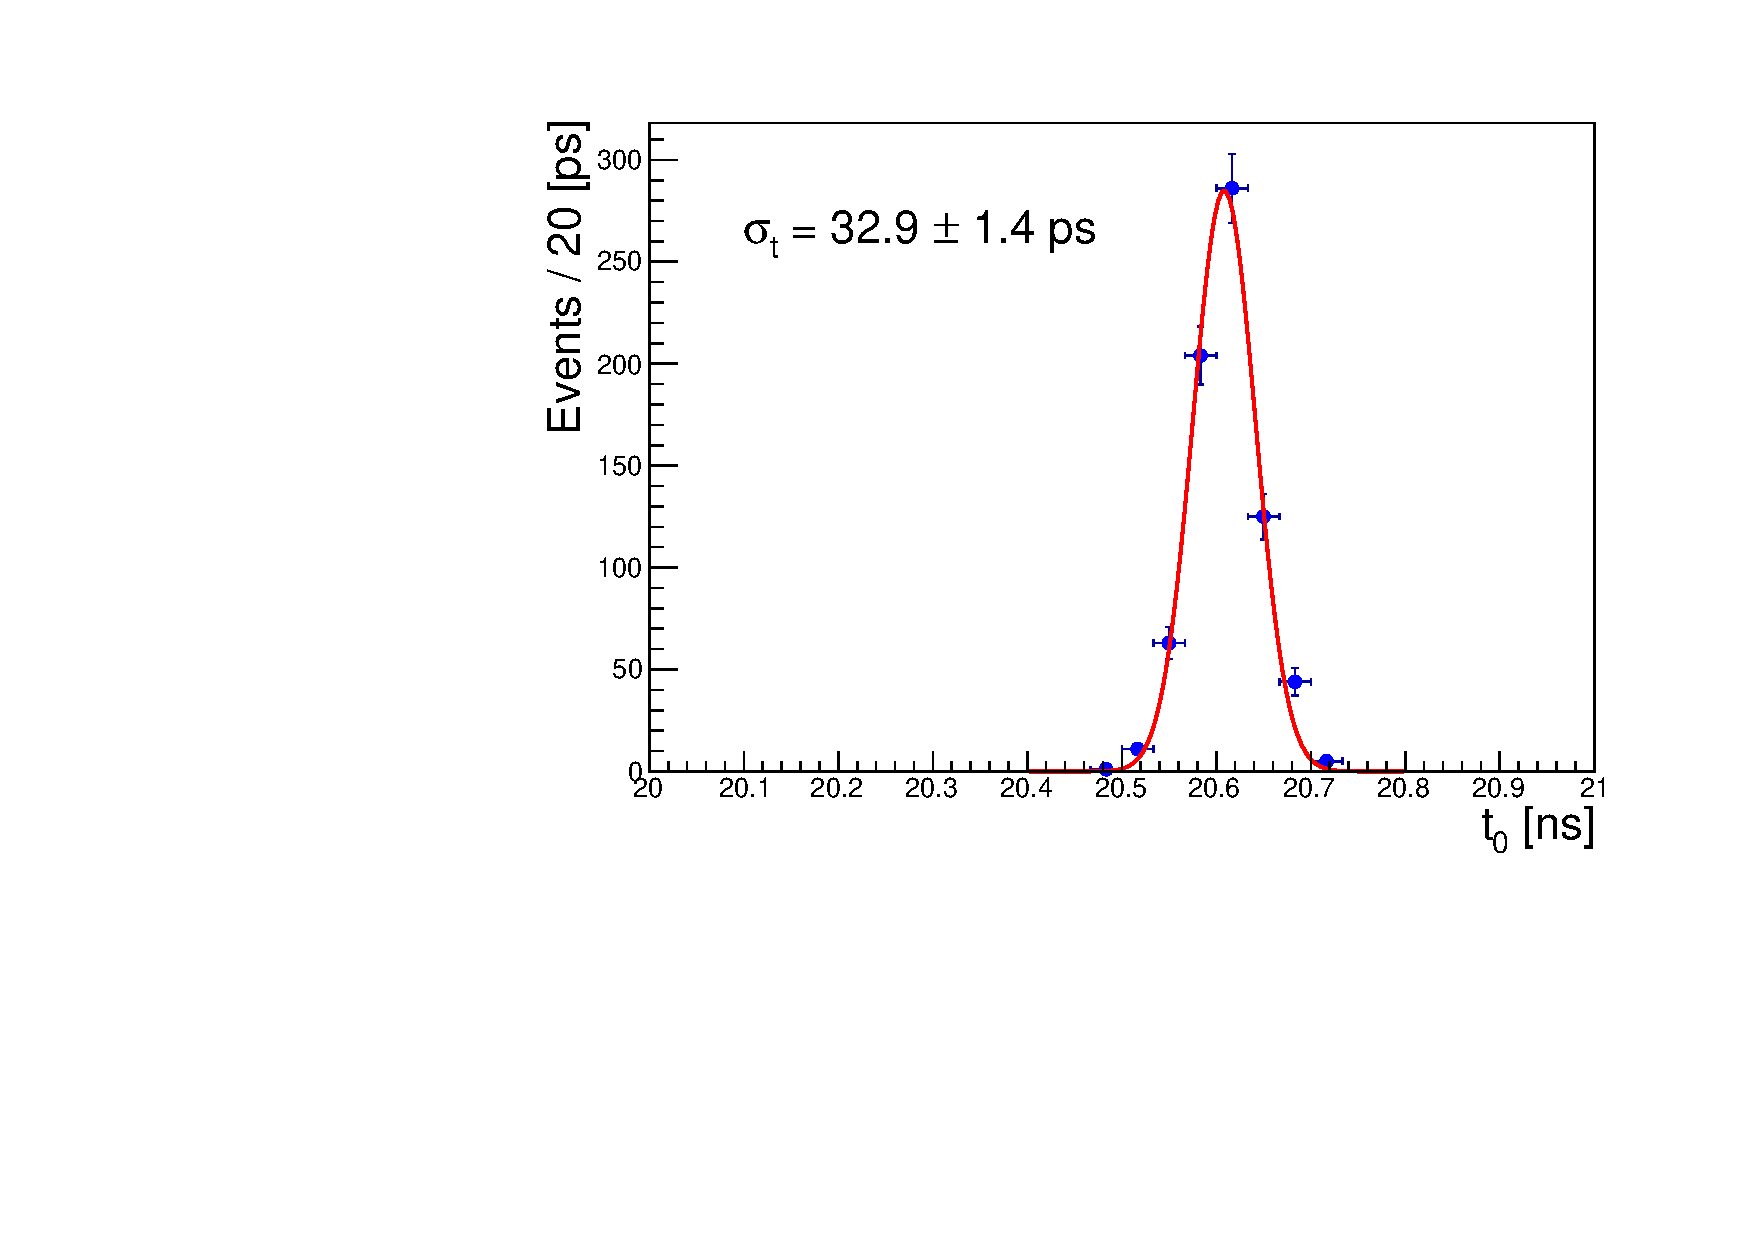
\includegraphics[width=0.48\textwidth]{figs/pre_rad_st_1ns_snr_30_cfd_tot_threshold_35_percent_v2.pdf}
    \caption{(Left) timestamp ($t_{0}$) distribution for a 30~\si{mV} threshold using a leading edge discriminator.
    (Right) timestamp ($t_{0}$) distribution for a 35\% threshold using a constant fraction discriminator. Both figures
    include the time-walk correction based on the measured ToT.
    Both figures use pre-radiated unprocessed pulses, a shaping time (ST) of 1~\si{ns}, and correspond to SNR of 30.}
    \label{fig:time_res}
  \end{figure}


\subsection{Time-walk correction and time-over-threshold}\label{sec:tw_and_tot}
A time-walk correction is applied in order to correct the timestamp drift of pulses with varying amplitudes~\cite{Spieler}.
The correction is based on the measured time-over-theshold: $\mathrm{ToT} = t_{1} - t_{0}$. As expected, we observe that the ToT correction
is large for the LE case and negligible for CF (see Fig.~\ref{fig:time_resolution_scan}).
Figure~\ref{fig:ToT} (left) shows a typical two dimensional map of $t_{0}$ and ToT for the
LE algorithm, wherein a clear correlation between $t_{0}$ and ToT is observed. 
We construct a profile graph of $t_{0}$ versus ToT by calculating the mean $t_{0}$ in
each bin of ToT as shown on the right of Figure~\ref{fig:ToT}, and then fit the profile graph to a 2nd-order polynomial to 
obtain the time-walk correction. The resulting analytical expression after the fit is then used to alleviate the dependence of $t_{0}$ on ToT.
The time-walk correction is expressed in Eq.~\ref{eq:time_walk}, where $p_{2}$ and $p_{1}$ are the quadratic
and linear coefficients of the 2nd-oder polynomial fit. Different corrections are derived for each simulation scenario
characterized by the values of the simulation parameters: ST, SNR, and LGAD irradiation level.
As shown in Fig.~\ref{fig:time_resolution_scan} (left) the effect of the time-walk depends on the threshold used and correcting for it
can yield significant improvements in the measured time resolution.

\begin{equation}\label{eq:time_walk}
  t_{0}^{\mathrm{corrected}} = t_{0}-(p_{2}\mathrm{ToT}^2+p_{1}\mathrm{ToT})
\end{equation}

\begin{figure}[htbp]
  \centering
  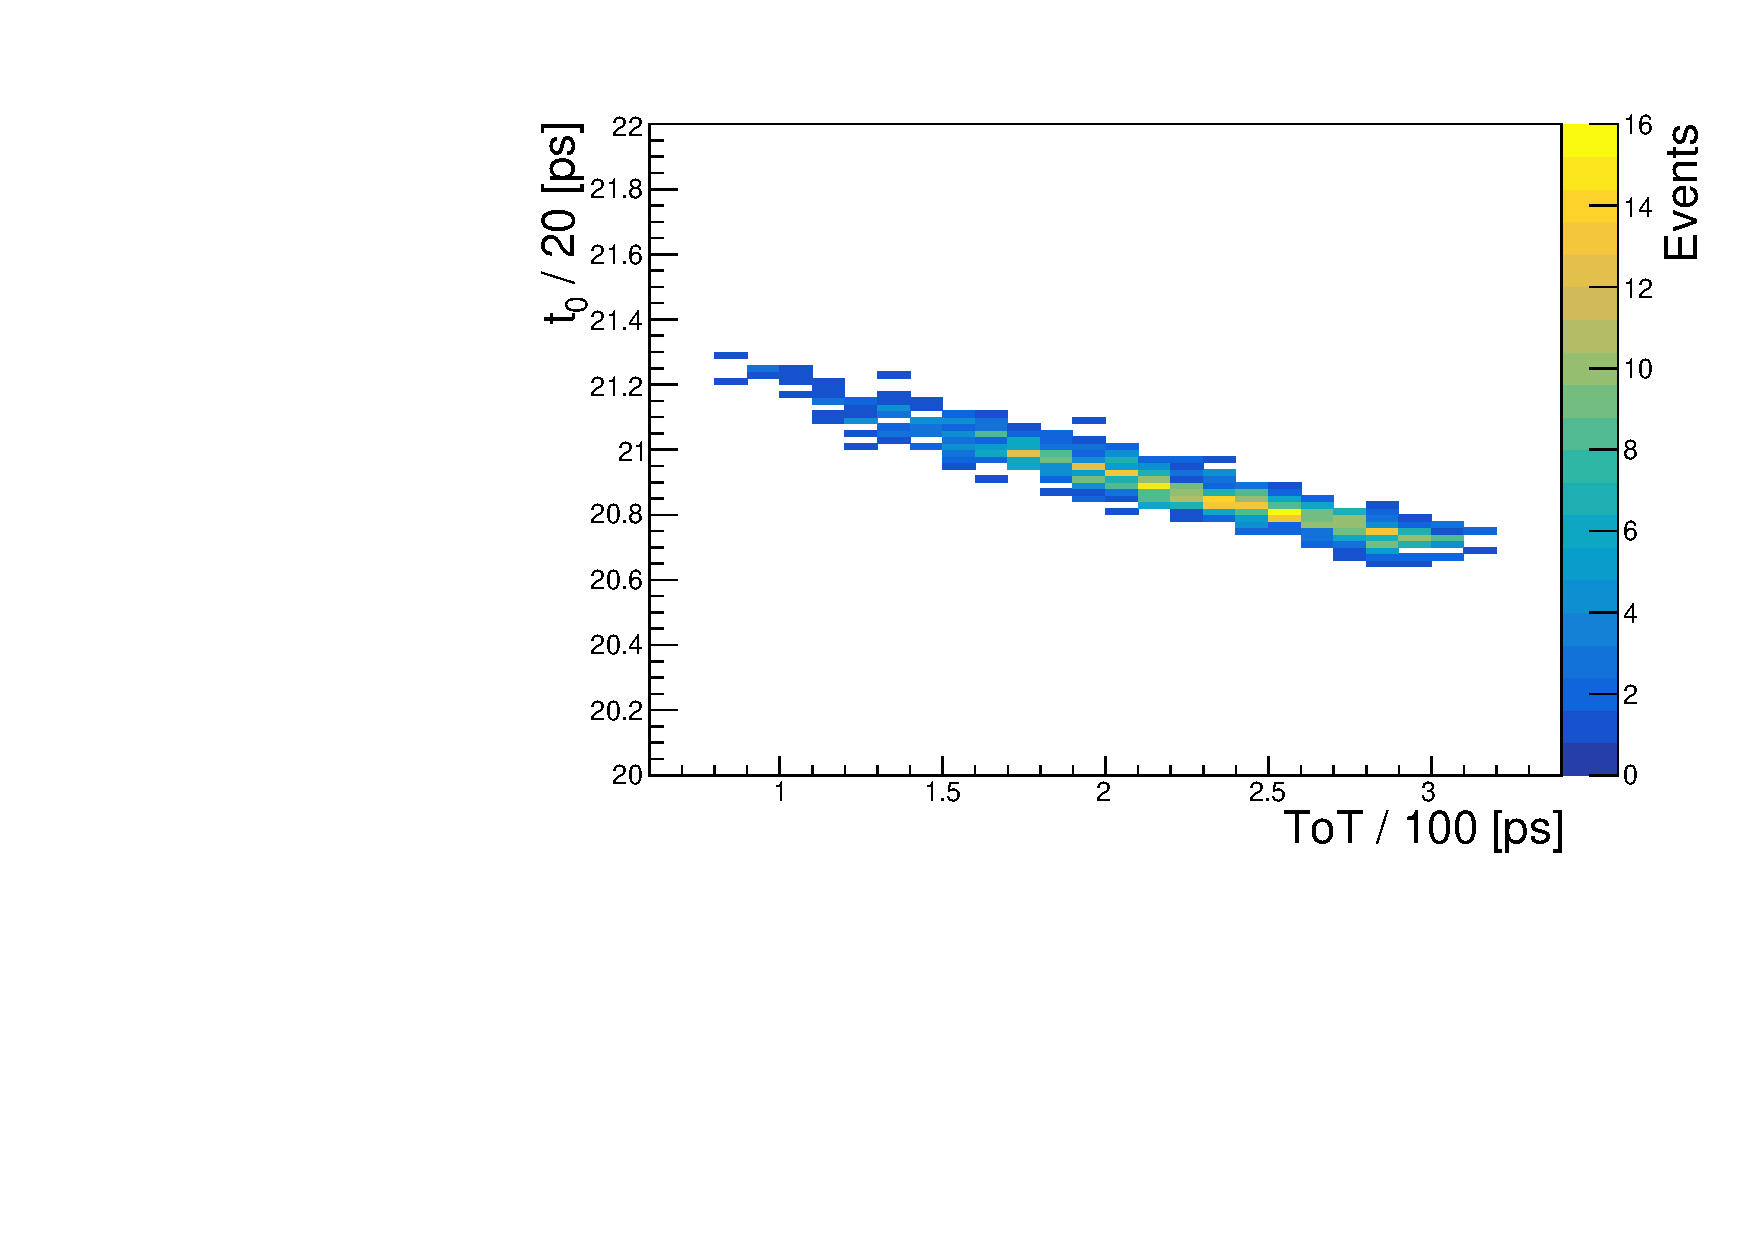
\includegraphics[width=0.48\textwidth]{figs/twoD_ToT_pre_rad_st_1ns_snr_30_le_tot_threshold_30mV_v2.pdf} \hfill
  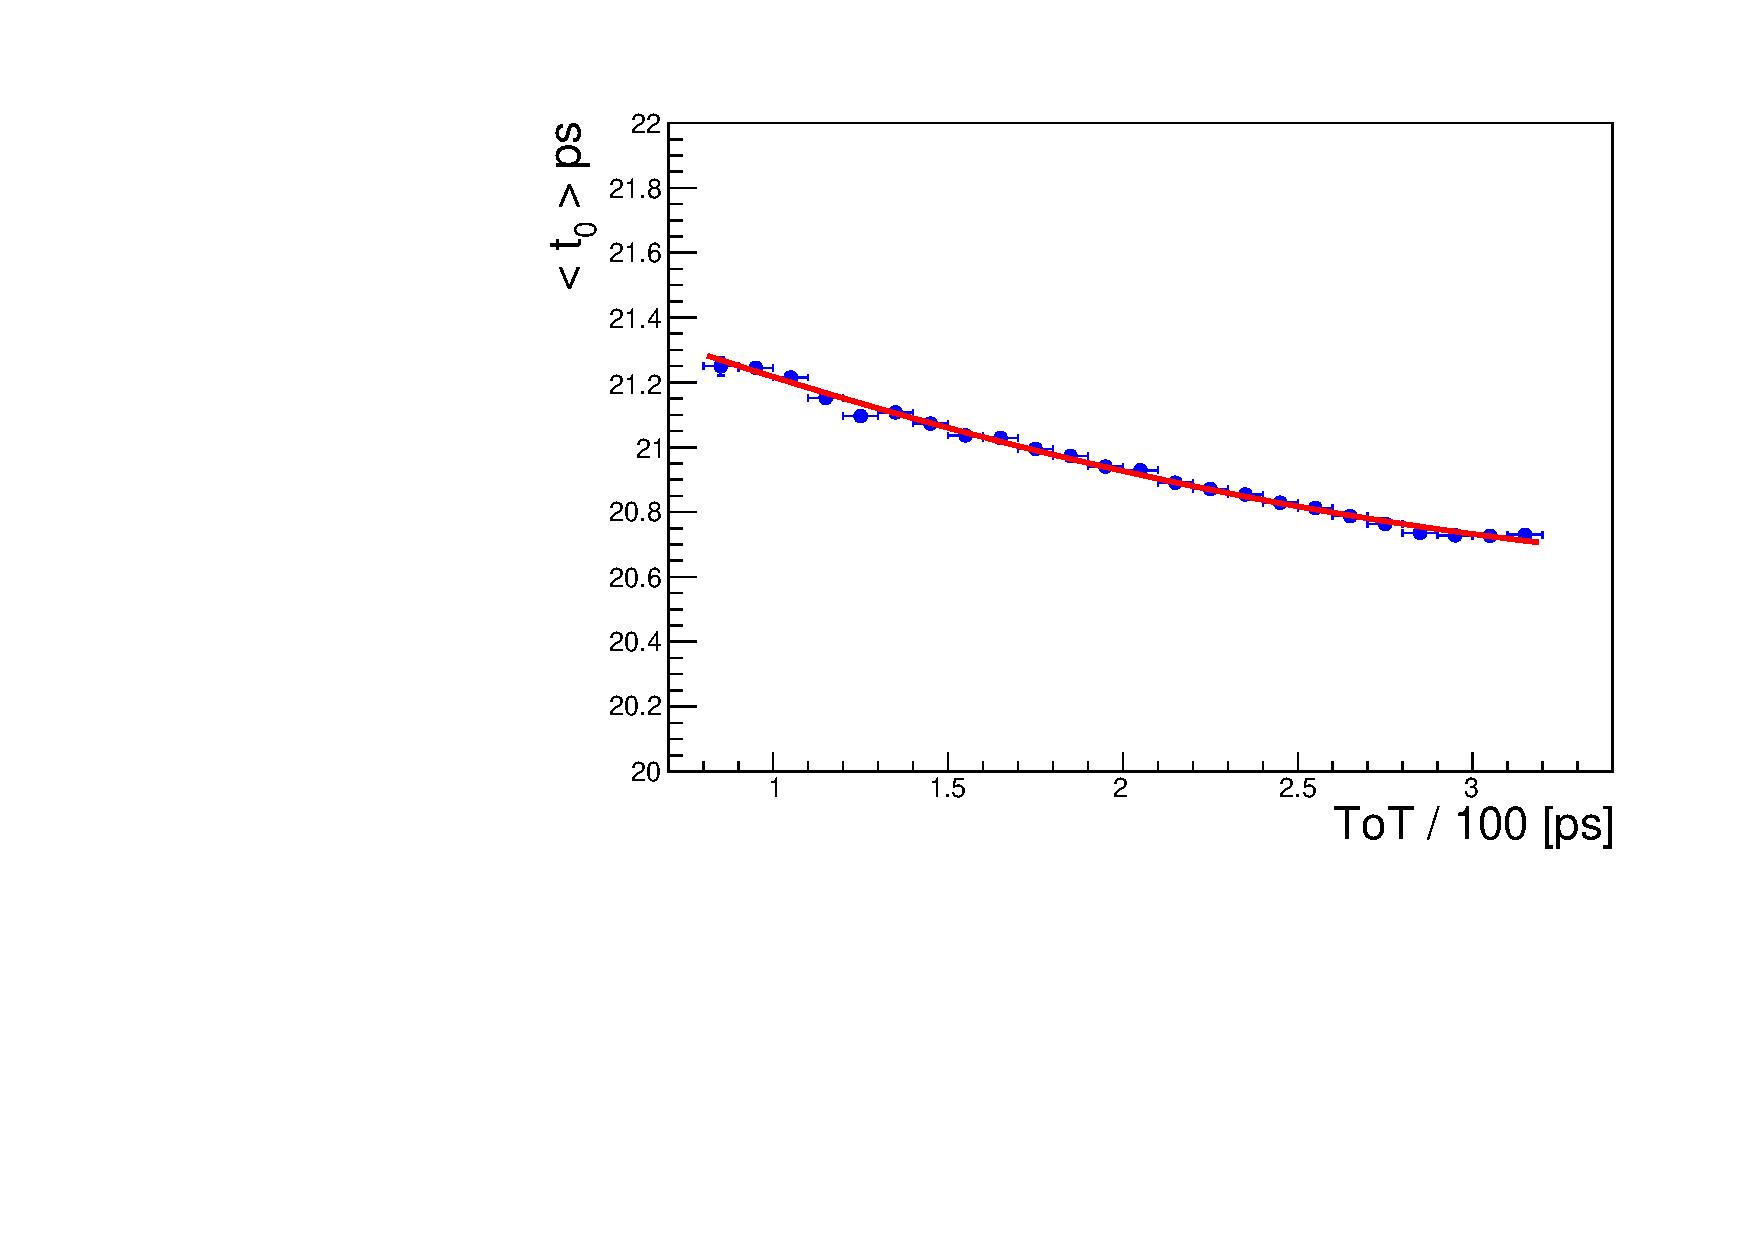
\includegraphics[width=0.48\textwidth]{figs/oneD_ToT_pre_rad_st_1ns_snr_30_le_tot_threshold_30mV_v2.pdf}
  \caption{(Left) two dimenasional map of the timestamp ($t_{0}$) and ToT ($t_{1} - t_{0}$).
  (Right) one dimensional projection of the timestamp ($t_{0}$) dependence on ToT, the red curve is the 2nd-order polinomial fit that
  ultimately is used to correct $t_{0}$. Both figures use a shaping time (ST) of 1~\si{ns} and correspond to a SNR of 30.}
  \label{fig:ToT}
\end{figure}




\section{LGAD Front-end Electronics Performance}\label{sec:results}

We discuss the studies of the FEE performance as a function of 
the shaping time and SNR in Sec.~\ref{sec:shaping_time} and 
the irradiation dose in Sec.~\ref{sec:rad_tolerance}.

\subsection{Front-end electronics shaping time and SNR studies}\label{sec:shaping_time}
We scan the ST of the FEE and the SNR. The results for the pre-irradiated LGAD sensor are summarized in Table.~\ref{tab:shaping_time_prerad},
where the CF results are from the \textit{ideal} implementation. The {\color{red} split-and-delay}
 and the \textit{ideal} CFD implementations are compatible within uncertainties thus we only use one table for those results.
 We observe that the best results are consistently obtained by the 0.5~\si{ns} and 1.0~\si{ns} STs regardless of the SNR. We observe that
 longer STs are more affected by less favorable SNR. For example, for an SNR of 20, the time resolution is ~37~\si{ps} and ~100~\si{ps} for a
ST of 0.5~\si{ns} and 4.0~\si{ns}, respectively. We note that CF consistently outperforms LE, and this effect is also observed
 for less favorable SNR and slower ST. Comparing CF and LE for the 1.0~\si{ns} ST with SNR of 20 yields a difference in performance of
 26~\si{ps}, when subtracted in quadrature. Additionally, we observe that time resolutions better than 25~\si{ps} could not be achieved which
 is consistent with the known intrinsic jitter of the LGAD sensor. The latter is taken into account by the WF2 simulation and
confirmed in our study. For a SNR of 1000, equivalent to having negligible noise, we obtained a time resolution consistent with 25~\si{ps}.
Finally, in the case of the pre-irradiated sensor we observed that time resolutions of ~35~\si{ps} are achievable for
STs between 0.5 - 1.0~\si{ns} and a SNR of 30.

The {\color{red} second order RC} CFD implementation shows a degradation on the time resolution when compared
to the {\color{red} split-and-delay}. Table.~\ref{tab:pcfd} shows the time resolution for the three SNR scenarios
studied for a 2~\si{ns} ST. We observe a 50~\si{ps} degradation for a SNR of 20 and  xx~\si{ps} degradation for a SNR of 100.

\begin{table}\label{tab:shaping_time_prerad}
    \begin{tabular}{c|ccc|ccc}
    \multicolumn{1}{c}{}& \multicolumn{6}{c}{Time Resolution (ps)} \\
    \multicolumn{1}{c}{}&\multicolumn{3}{c}{Leading Edge} & \multicolumn{3}{c}{Constant Franction}\\ \hline
    ST (ns) & SNR = 20   & SNR = 30      & SNR = 100     & SNR = 20      & SNR = 30      & SNR = 100 \\
    0.5 & $38$    & $35$  & $29$  & $37$  & $35$  & $30$ \\
    1.0 & $45$    & $37$  & $29$  & $36$  & $33$  & $26$ \\
    2.0 & $63$    & $48$  & $31$  & $48$  & $34$  & $29$ \\
    4.0 & $103$  & $75$  & $38$  & $74$  & $55$  & $32$ \\
    \end{tabular}
    \caption{50~$\mu$m pre-radiation LGAD sensor simulation: summary of best time resolution obtained for SNRs
    of 20, 30, and 100. Leading edge and constant fraction results are shown.}
 \end{table}


 \begin{table}\label{tab:shaping_time_prerad_psCFD}
   \begin{center}
     \begin{tabular}{c|ccc}
     \multicolumn{1}{c}{}& \multicolumn{3}{c}{Time Resolution (ps)} \\
     \multicolumn{1}{c}{}& \multicolumn{3}{c}{$\mathrm{(RC)}^{2}$ Constant Fraction}\\ \hline
     ST (ns) & SNR = 20      & SNR = 30      & SNR = 100 \\
     1.0 & $58$  & $ 40$  & $28$ \\
     2.0 & $68$  & $ 49$  & $30$ \\     
     \end{tabular}
     \caption{50~$\mu$m pre-radiation LGAD sensor using a second order RC implementation of a CFD.
     Summary of best time resolution obtained using a ST of 2\si{ns} for SNRs of 20, 30, and 100.}
   \end{center}
  \end{table}

 \begin{table}\label{tab:shaping_time_5e14}
     \begin{tabular}{c|ccc|ccc}
     \multicolumn{1}{c}{}& \multicolumn{6}{c}{Time Resolution (ps)} \\
     \multicolumn{1}{c}{}&\multicolumn{3}{c}{Leading Edge} & \multicolumn{3}{c}{Constant Franction}\\ \hline
     ST (ns) & SNR = 20   & SNR = 30      & SNR = 100     & SNR = 20      & SNR = 30      & SNR = 100 \\
     0.5 & $37$  & $32$  & $26$  & $33$  & $31$  & $25$ \\
     1.0 & $41$  & $34$  & $29$  & $33$  & $31$  & $26$ \\
     2.0 & $57$  & $45$  & $30$  & $44$  & $37$  & $24$ \\
     4.0 & $93$  & $68$  & $37$  & $71$  & $52$  & $30$ \\
     \end{tabular}
     \caption{50~$\mu$m LGAD sensor simulation after neutron fluence of
      $5\times 10^{14}$~n/cm$^2$: summary of best time resolution obtained for SNRs
     of 20, 30, and 100. Leading edge and constant fraction results are shown.}
  \end{table}

 \begin{table}\label{tab:shaping_time_5e14_psCFD}
     \begin{tabular}{c|ccc|ccc}
     \multicolumn{1}{c}{}& \multicolumn{3}{c}{Time Resolution (ps)} \\
     \multicolumn{1}{c}{}& \multicolumn{3}{c}{$\mathrm{(RC)}^{2}$ Constant Fraction}\\ \hline
     ST (ns) & SNR = 20      & SNR = 30      & SNR = 100 \\
     1.0 & $55$  & $ 37$  & $30$ \\
     2.0 & $70$  & $ 53$  & $33$ \\     
     \end{tabular}
     \caption{50~$\mu$m LGAD sensor simulation after neutron fluence of
      $5\times 10^{14}$~n/cm$^2$ using a second order RC implementation of a CFD. 
      Summary of best time resolution obtained for SNRs
     of 20, 30, and 100. }
  \end{table}




  \begin{table}\label{tab:shaping_time_1e_15}
      \begin{tabular}{c|ccc|ccc}
      \multicolumn{1}{c}{}& \multicolumn{6}{c}{Time Resolution (ps)} \\
      \multicolumn{1}{c}{}&\multicolumn{3}{c}{Leading Edge} & \multicolumn{3}{c}{Constant Franction}\\ \hline
      ST (ns) & SNR = 20   & SNR = 30      & SNR = 100     & SNR = 20      & SNR = 30      & SNR = 100 \\
      0.5 & $48$    & $38$    & $27$  & $42$    & $34$  & $24$ \\
      1.0 & $60$    & $47$    & $28$  & $47$    & $37$  & $23$ \\
      2.0 & $90$    & $68$    & $32$  & $65$    & $50$  & $27$ \\
      4.0 & $147$  & $109$  & $43$  & $119$  & $84$  & $34$ \\
      \end{tabular}
      \caption{50~$\mu$m LGAD sensor simulation after neutron fluence of
       $1\times 10^{15}$~n/cm$^2$: summary of best time resolution obtained for SNRs
      of 20, 30, and 100. Leading edge and constant fraction results are shown.}
   \end{table}


 \begin{table}\label{tab:shaping_time_1e15_psCFD}
     \begin{tabular}{c|ccc|ccc}
     \multicolumn{1}{c}{}& \multicolumn{3}{c}{Time Resolution (ps)} \\
     \multicolumn{1}{c}{}& \multicolumn{3}{c}{$\mathrm{(RC)}^{2}$ Constant Fraction}\\ \hline
     ST (ns) & SNR = 20      & SNR = 30      & SNR = 100 \\
     1.0 & $45$  & $ 39$  & $29$ \\
     2.0 & $83$  & $ 53$  & $33$ \\     
     \end{tabular}
     \caption{50~$\mu$m LGAD sensor simulation after neutron fluence of
      $1\times 10^{15}$~n/cm$^2$ using a second order RC implementation of a CFD. 
      Summary of best time resolution obtained for SNRs
     of 20, 30, and 100. }
  \end{table}
  
  
\subsection{Timing performance as a function of irradiation}\label{sec:rad_tolerance}
We study the effect of irradiation on the time resolution of a 50~$\mu$m LGAD sensor. The impact of irradiation on the unprocessed
signal pulse shapes are accounted for by the WF2 simulation. We consider three cases: pre-irradiated, and neutron fluences of
$5\times 10^{14}$~n/cm$^2$ and $1\times 10^{15}$~n/cm$^2$. We perform the same studies as in the pre-irradiated case discussed in
Sec.~\ref{sec:shaping_time}. The results for the irradiated LGAD are presented in Tab.~\ref{tab:shaping_time_5e14} and
Tab.~\ref{tab:shaping_time_1e_15} for neutron fluences of
$5\times 10^{14}$~n/cm$^2$ and $1\times 10^{15}$~n/cm$^2$, respectively.
We observe similar trends to those of the pre-radiation sensor described in
Sec.~\ref{sec:shaping_time}. We note that when using STs between 0.5 - 1.0~\si{ns} and a SNR of 30, time resolutions of the order
of ~31~\si{ps} and ~37~\si{ps} are obtained for $5\times 10^{14}$~n/cm$^2$ and $1\times 10^{15}$~n/cm$^2$, respectively.

\section{Conclusion}\label{sec:conclusion}


We study the time resolution of a 50~$\mu$m Low-gain avalanche diode (LGAD) sensor using a simulation framework that includes the
modeling of the raw unprocessed LGAD signal pulse, the front-end electronics, and effects of analog-to-digital converter resolution.
We used a second order low-pass filter to model the front-end electronics. 
We focus on the shaping time (ST) and signal-to-noise ratio (SNR) of the front-end electronics and its interplay
with the irradiation level of the sensor. We reproduce the known LGAD jitter of ~25~\si{ps}
for fast STs and large SNRs. We observe a clear degradation of the time resolution with SNR and slower STs. The best results are
obtained using a ST of 0.5~\si{ns} and using constant fraction (CF) discriminator, and similar results are obtained with a ST of 1.0~\si{ns}. For a SNR of 30
and for STs between 0.5-1.0~\si{ns} we obtain time resolutions between ~30 - 37~\si{ps} for the 3 irradiations considered. The
reduction in gain with irradiation could bring the SNR for the most irradiated LGAD ($1\times 10^{15}$~n/cm$^2$) to 20 and thus
worsen the time resolution to ~42 - 47~\si{ps}. We note a clear gain in performance of CF over leading edge (LE) discriminators, particularly at
low SNR and the largest irradiation level. For an ST of 1.0~\si{ns} at SNR = 30, the performance improvement of CF over LE
is ~26\si{ps} for the pre-irradiated sensor and ~37\si{ps} for the irradiated sensor with neutron fluence of
$1\times 10^{15}$~n/cm$^2$. A performance degradation is observed when using a {\color{red}second order RC} implementation of the CFD,
especially at lower SNRs. Overall our simulation results indicate that time resolutions better than
45~\si{ps} are achievable for a 50~$\mu$m LGADs for irradiation levels up to neutron fluences of $1\times 10^{15}$~n/cm$^2$.


\section*{Acknowledgment}

%We thank the FTBF personnel and Fermilab accelerator's team for very good beam
%conditions during our test beam time. We also appreciate the technical support
%of the Fermilab SiDet department for the rapid production of wire-bonded and
%packaged LGAD assemblies. We would like to thank Alan Prosser and Ryan Rivera
%or their critical help in setting up the DAQ and trigger chain. We thank Ned
%Spencer, Max Wilder, and Forest McKinney-Martinez for their technical
%assistance, and the CNM and HPK manufacturing team. We acknowledge the help of
%V. Cindro and I. Mandic with the neutron irradiations.

A. Apresyan gratefully acknowledges support from DOE Early Career Research Program.

This document was prepared using the resources of the Fermi National Accelerator
Laboratory (Fermilab), a U.S. Department of Energy, Office of Science, HEP User
Facility. Fermilab is managed by Fermi Research Alliance, LLC (FRA), acting
under Contract No. DE-AC02-07CH11359. Part of this work was performed within the
framework of the CERN RD50 collaboration.

This work was supported by the Fermilab LDRD 2017.027 {\color{red} (Cristian: did Artur ask to include LDRD here?)}; by the United States
Department of Energy grant DE-FG02-04ER41286; by the California Institute of
Technology High Energy Physics under Contract DE-SC0011925; by the European
Union's Horizon 2020 Research and Innovation funding program, under Grant
Agreement no. 654168 (AIDA-2020) and Grant Agreement no. 669529 (ERC
UFSD669529); by the Italian Ministero degli Affari Esteri and INFN Gruppo V; and
by the Spanish Ministry of Economy, Industry and Competitiveness through the
Particle Physics National Program (ref. FPA2014-55295-C3-2-R and
FPA2015-69260-C3-3-R) co-financed with FEDER funds.


% The Appendices part is started with the command \appendix;
% appendix sections are then done as normal sections

%\appendix
%\section{Appendix A}



% \section{}
% \label{}

%% If you have bibdatabase file and want bibtex to generate the
%% bibitems, please use
%%
%%  \bibliographystyle{elsarticle-num}
%%  \bibliography{<your bibdatabase>}

%% else use the following coding to input the bibitems directly in the
%% TeX file.

\bibliography{lgad_frontend_simulation}{}
\bibliographystyle{ieeetr}

%\begin{thebibliography}{00}

%% \bibitem{label}
%% Text of bibliographic item

%\bibitem{}

%\end{thebibliography}
\end{document}
\endinput
%%
%% End of file `elsarticle-template-num.tex'.
